\documentclass[nobuilddate,nochap]{Docencia}

\title{Matemáticas II - Apuntes de clase}
\author{Departamento de Matemáticas}
\date{2019-2020}


\usepackage{tikz}
\usepackage{tikz-3dplot}
\usepackage{fancysprefs}
\usepackage{svg}
\usepackage{xfp}
\usepackage{float}



\usetikzlibrary{calc,patterns,angles,quotes}

\newcommand{\crossprod}[6]{\ensuremath{\left|\begin{matrix}\vec{i}&\vec{j}&\vec{k}\\#1&#2&#3\\#4&#5&#6\end{matrix}\right|}}
\newcommand{\crossprodcalc}[6]{\fpeval{#2*#6-#3*#5}\vec{i} - \fpeval{#1*#6-#3*#4}\vec{j}+\fpeval{#1*#5-#2*#4}\vec{k}}
\newcommand{\crossprodcalcvec}[6]{\left(\fpeval{#2*#6-#3*#5}, \fpeval{-(#1*#6-#3*#4)},\fpeval{#1*#5-#2*#4}\right)}
\newcommand{\crossprodandcalc}[6]{\crossprod{#1}{#2}{#3}{#4}{#5}{#6}=\crossprodcalc{#1}{#2}{#3}{#4}{#5}{#6}=\crossprodcalcvec{#1}{#2}{#3}{#4}{#5}{#6}}
\newcommand{\detwrite}[9]{\left|\begin{matrix}#1&#2&#3\\#4&#5&#6\\#7&#8&#9\end{matrix}\right|}
\newcommand{\detwritecalc}[9]{
(\fpeval{+#1*#5*#9})+
(\fpeval{+#2*#6*#7})+
(\fpeval{+#3*#4*#8})
-(\fpeval{#3*#5*#7})
-(\fpeval{#1*#6*#8})
-(\fpeval{#2*#4*#9})
=\fpeval{(#2*#6-#3*#5)*#7 - (#1*#6-#3*#4)*#8+ (#1*#5-#2*#4)*#9}}
\newcommand{\detcalc}[9]{\fpeval{(#2*#6-#3*#5)*#7 - (#1*#6-#3*#4)*#8+ (#1*#5-#2*#4)*#9}}
\renewcommand{\ve}[1]{\ensuremath{\mathbf{#1}}}
\newcommand{\vi}{\vec{i}}
\newcommand{\vj}{\vec{j}}
\newcommand{\vk}{\vec{k}}
\newcommand{\vw}{\vec{w}}
\newcommand{\ud}[0]{\mathrm{d}}
\newcommand{\lgdlp}{Lugar geométrico de los puntos del espacio que equidistan de}


\tikzset{
    vector/.style = {
        thick,
        > = stealth',
    },
    axis/.style = {
        very thin,
        > = stealth',
    },
}


\begin{document}

\pagestyle{plain}
\maketitle
\tableofcontents
\newpage

\newcommand{\hide}[1]{#1}

\renewcommand{\vec}[1]{\overrightarrow{#1}}

% \paragraph{Introducción}

% \begin{itemize}
%     \item 2º de Bachillerato no es un curso para preparar la EVAU. Es un curso orientado a la universidad y es para eso para lo que te vamos a preparar. 
%     %
%     Ya tendremos tiempo a final de curso para preparar la EVAU.

%     \item Temario muy extenso (¿Aquí también? Sí hijo sí...). Cuidado.
    
%     \item 2º de Bachillerato no es solo estudiar. Sed responsables y organizados para poder disfrutar del curso. ¡Tratad bien a vuestras familias! Que los exámenes no os hagan ser unos amargados.
    
%     \item A vuestra disposición por correo y por el classroom para lo que necesitéis. Colgaremos en el classroom los enunciados de los exámenes, las soluciones, etc.

%     \item Metodología de clase.
    
%     \item Criterios de evaluación.

%     \subitem 10\%, 30\%, 60\%. Estudiar al día. Tutorías a demanda. Cosas que tenéis que saber, aunque, seminarios.

%     \subitem Pruebecita del lunes, tal vez con teoría.

% \end{itemize}

\chapter{Probabilidad y Estadística}

\section{Probabilidad}
% Página 67 del cuaderno en papel

Los sucesos en probabilidad se escriben entre comillas y se representan con una letra mayúscula.

\begin{itemize}
    \item[m] $I =$ impar
    \item[m] $I =$ probabilidad de sacar un número impar
    \item[m] $I =$ "Probabilidad de sacar un número impar"
    \item[b] $I =$ "Sacar un número impar"
\end{itemize}

\textbf{Operaciones con conjuntos (o sucesos)}

$A\cup B = \{x\in A \vee x \in B\}$ (Unión)

$A\cap B = \{x\in A \wedge x \in B\}$ (Intersección - Probabilidad compuesta)

$A^c = \overline{A} = \{x\not\in A$ (Complementario) \textit{No se llama contrario}.

$A - B = \{x\in A \wedge x \not\in B\}$ (Diferencia)

\obs $A - B = A \cap \overline{B}$

\begin{defn}[Leyes\IS de de Morgan]
\[\overline{A\cap B} = \overline{A}\cup \overline{B}\]
\[\overline{A\cup B} = \overline{A}\cap \overline{B}\]
\end{defn}



\begin{defn}[Compatibilidad]
Sean $A,B$ dos sucesos.

Son compatibles si $A\cap B \not= \emptyset$. 
Son incompatibles si $A\cap B =\emptyset$
\end{defn}

\begin{defn}[Sistema completo de sucesos]
Sean $A_1,...,A_n$ sucesos de un cierto experimento aleatorio.
%
Se dice que forman un sistema completo de sucesos del espacio muestral $E$ cuando:

\begin{itemize}
    \item $\displaystyle\bigcup_{i=1}^n A_i = A_1\cup A_2 \cup ... \cup A_n =  E$
    \item $A_i\cap A_j = \emptyset\;\;\; \forall i,j=1...n$
\end{itemize}
\end{defn}

\begin{example}
Sea $E = \{1,2,3,4,5,6\}$. ¿Son sistemas completos de sucesos las siguientes agrupaciones?

\begin{itemize}
    \item $A_1 = \{1,2,3\}; A_2 = \{4,5\} ; A_3 = \{6\}$
    \item $A_1 = \{\text{múltiplos de 3}\} ; A_2 = \{\text{números pares}\} ; A_3 = \{1,5\}$
\end{itemize}
\end{example}


\begin{prop}Sea $A_1,...,A_n$ un sistema completo de sucesos. Entonces \[\displaystyle\sum_{i=1}^n P(A_i) = 1\]
\end{prop}


\begin{defn}[Regla de Laplace]
Si los socesos elementales de un experimento aleatorio son equiprobables, entonces, $P(A) = \frac{\text{casos favorables}}{\text{casos posibles}}$
\end{defn}
\obs ¿Y si no son equiprobables? 

\begin{defn}[Probabilidad\IS Ley de los grandes números]
Sea $A$ un suceso y $h(A)$ su frecuencia de ocurrencia relativa\footnote{El porcentaje de veces que ese suceso ocurre.} en $n$ repeticiones del experimento. Entonces \[P(A) = \lim_{n\leftrightarrow \infty}h(A)\]
\end{defn}


\begin{defn}[Probabilidad\IS Axiomática de Kolmogorov]
    Sea $p$ una función que asocia a cada suceso $A$ del espacio de sucesos $S$ un número real designado por $p(A)$.
    
    Decimos que $p$ es una probabilidad si cumple las siguientes propiedades:
    \begin{itemize}
        \item $0\leq p(A) \leq 1 \;\;\;\forall A\in S$
        \item $p(E) = 1$
        \item $A\cap B = \emptyset \implies p(A\cup B) = p(A) + p(B)$
    \end{itemize}
\end{defn}

\paragraph{Propiedades de la probabilidad:} Sea $A$ un suceso cualquiera:
\begin{itemize}
    \item $P(\overline{A}) = 1 - P(A)$
    \item $A\subset B \implies P(A) \leq P(B)$
    \item $0\leq P(A) \leq 1$
    \item $P(A\cup B) = P(A) + P(B) - P(A\cap B)$
\end{itemize}

\begin{center}
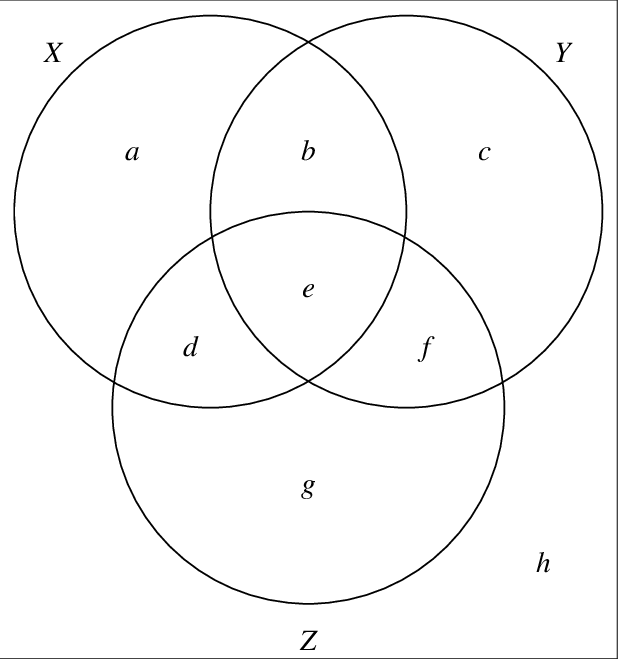
\includegraphics[scale=0.3]{img/Venn-diagram-visualization-of-a-3-event-probability-space-O.png}
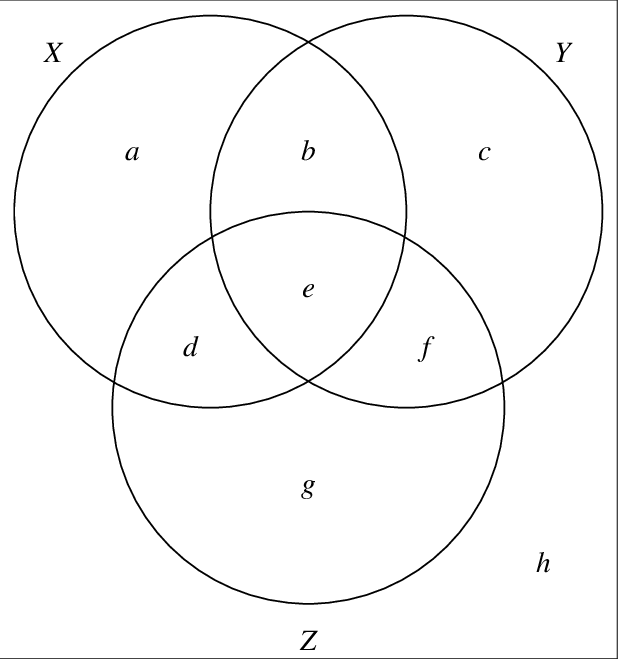
\includegraphics[scale=0.3]{img/Venn-diagram-visualization-of-a-3-event-probability-space-O.png}
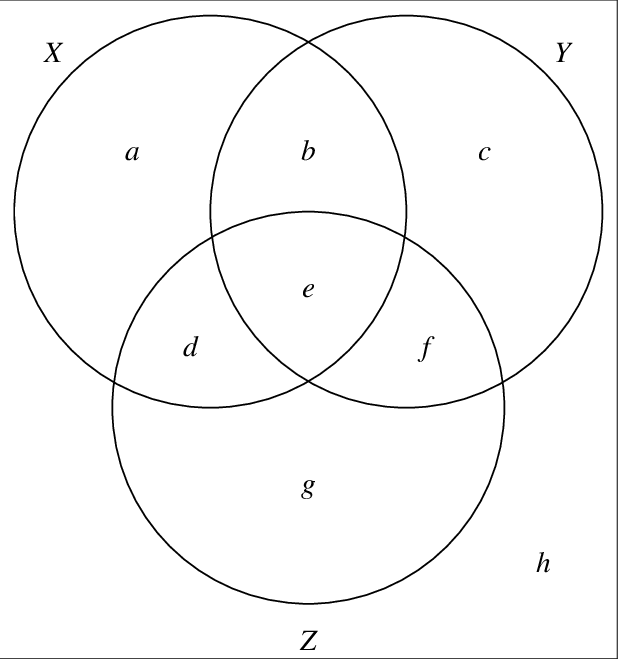
\includegraphics[scale=0.3]{img/Venn-diagram-visualization-of-a-3-event-probability-space-O.png}
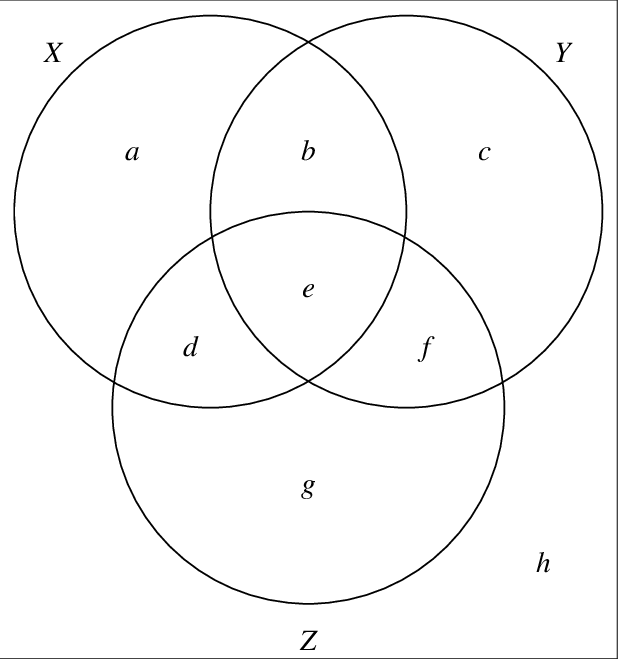
\includegraphics[scale=0.3]{img/Venn-diagram-visualization-of-a-3-event-probability-space-O.png}
\end{center}

\begin{defn}[Probabilidad\IS condicionada]
Sean $A,B$ sucesos de un suceso aleatorio. 

Se define la probabilidad condicionada $p(A/B)$ como la probablidad de que se produzca $A$ si sabemos que se ha producido $B$.

\[P(A/B) = \frac{P(A\cap B)}{P(B)}\]
\end{defn}

\textit{Este es un buen momento para hacer algún ejercicio. Página 349, ejer 36 por ejemplo. Recordamos que $P(A\cup B) = P(A) + P(B) - P(A\cap B)$}

\begin{defn}[Independencia de sucesos]
$A,B$ son sucesos independientes si y sólo si \[P(A/B) = P(A/\overline{B}) = P(A)\]
\end{defn}

\begin{theorem}
\[A,B \text{ independientes } \dimplies P(A\cap B) = P(A)·P(B)\]
\end{theorem}
\begin{proof}
\[\left.\begin{array}{c}
P(A/B) = \frac{P(A\cap B)}{P(B)} \dimplies P(A\cap B) = P(B)·P(A/B)\\A,B \text{ independientes } \dimplies P(A/B) = P(A)\end{array}\right\}*\]
\[(*) \implies P(A\cap B) = P(B)·\underset{P(A/B)}{P(A)} = P(B)·P(A)\]
\end{proof}

\begin{theorem}[Teorema\IS Probabilidad Total]
Sea $A_1,A_2,...,A_n$ un sistema completo de sucesos y sea $B$ otro suceso.
\[  
    P(B) = P(A_1\cap B) + P(A_2\cap B) + ... + P(A_n\cap B) = 
\]
\[
    P(B/A_1)·P(A_1) + P(B/A_2) · P(A_2) + ... + P(B/A_n)·P(A_n)
\]
\end{theorem}
\begin{theorem}[Teorema\IS de Bayes]
\[P(B/A) = \frac{P(A/B)·P(B)}{P(A)}\]
\end{theorem}
\begin{proof}
\[
\left.
\begin{array}{c}
    P(A\cap B) = P(A)·P(B/A)\\
    P(A\cap B) = P(B)·P(A/B)
\end{array}\right\} \implies P(A)·P(B/A) =  P(B)·P(A/B) \dimplies \]\[\dimplies P(B/A) = \frac{P(A/B)·P(B)}{P(A)} 
\]
\end{proof}


\paragraph{Bayesian trap (obtenido de youtube.com/Veritasium)}

\begin{example}
Se sabe que una enfermedad rara sólo afecta al 1\% de la población. 
%
El porcentaje de falsos positivos de las pruebas médicas es del 10\%, y el porcentaje de falsos negativos es del 1\%.

Intuitivamente, ¿cuál dirías que es la probabilida de tener la enfermedad sabiendo que has dado positivo en el test? ¿Podrías calcularlo numéricamente?

Los datos son: $P(E) = 0.01$, $P(-|E) = 0.01$ y $P(+|\overline{E})=0.1$

Aplicando el teorema de Bayes:

\[P(E|+) = \frac{P(+|E)·P(E)}{P(+)} = \frac{P(+|E)·P(E)}{P(+|E)·P(E) + P(+|\overline{E})·P(\overline{E})}= 0.01 \]
\end{example}


\section{Estadística}

A la hora de hacer un estudio estadístico buscamos obtener información sobre toda la población. A veces, esa cantidad de información es inmanejable e inconseguible. 
%
Por ejemplo, test de COVID a toda la población para ver cuántos lo han pasado, no es viable. 
%
Por ello, se selecciona una parte de la población y se le hacen los test a una parte para después extrapolar esos resultados.

Así, definimos:

\begin{defn}[Población]
\end{defn}

\begin{defn}[Muestra]
\end{defn}

\begin{defn}[Individuo]
\end{defn}

\textit{Nota: estos términos también se utilizan al tratar de tornillos en una fábrica.}

Este año vamos a trabajar y a distinguir los \concept[Parámetros\IS poblacionales]{parámetros poblacionales} de los \concept[Parámetros\IS muestrales]{muestrales}.
%
Llamaremos $\mu$ y $\sigma·$ a la media y desviación típica \emph{poblacionales} y $\bar{x}$ y $S$ a la media y desviación típica \emph{muestral}.

El \textbf{objetivo} de este tema es conseguir información sobre los parámetros poblacionales a partir de los parámetros muestrales. 

Para ello, antes de empezar es necesario que intentemos contestar la pregunta: ¿Cómo se asegura uno de que su muestra es buena? Porque si queremos saber lo que opinan los alumnos del colegio sobre la semipresencialidad y tomamos de muestra a los alumnos de 2º de Bachillerato, la información que saquemos no será fiable.

Necesitaremos que las muestras sean \concept[Representatividad de una muestra]{representativas} de toda la población, esto es, que refleje fielmente las características de la población.
%
Llamamos \concept{muestreo} al proceso por el que se construye una muestra de una población. 
%
Como seguro que te imaginas, hay distintos tipos de \textit{muestrear} una población. Vamos a verlos:

\subsection{Tipos de muestreo}

Los muestreos pueden ser aleatorios (si todos sus miembros tienen la misma posibilidad de ser elegidos) o no aleatorios (si no es así).
%
Dado que los muestreos aleatorios otorgan una mayor representatividad, nos centraremos en ellos:

Consideremos que eres el encargado de calidad de una fábrica de tornillos, que fabrica tornillos de distintos tipos.

\begin{itemize}
    \item Aleatorio simple.
        \subitem ¿Cuántas muestras se pueden formar?
        \subitem Estimación de los parámetros poblacionales desde los muestrales.
        \subitem Con reposición (días de la semana que se tienen que elegir), sin reposición (personas).
    \item Sistemático.
    \subitem Ordenados, de h en h (\concept{Constante de elevación}).
    \item Estratificado:
    \subitem Agrupación por característica. Estratos diferentes entre ellos. Elementos iguales en cada estrato.
    \subitem Afijación igual o proporcional.
    \subitem Dentro de cada estrato... ¿Aleatorio simple? ¿Sistemático?
    \item Conglomerados:
    \subitem División de cada característica. Conglomerados iguales entre ellos. Elementos diferentes en cada estrato.
    \subitem Dentro de cada estrato... ¿Aleatorio simple? ¿Sistemático?
\end{itemize}


\textbf{Importancia de los grupos control}

\section{Distribuciones de probabilidad}

Repaso de la distribución normal desde el PPT del departamento.
% 
\section{Inferencia estadística}

Inferir significa deducir algo o sacarlo como conclusión de otra cosa. \footnote{\href{https://dle.rae.es/inferir}{https://dle.rae.es/inferir}}

La tarea que nos va a mantener ocupados unas semanas va a ser la siguiente: \textit{Disponemos de una población con un parámetro desconocido. Tomaremos una muestra e inferiremos acerca del valor del parámetro poblacional utilizando información sobre la muestra.}


\subsection{Inferencia sobre la media}

Trabajaremos haciendo inferencia de la media. 
%
Tendremos poblaciones de las que conocemos su desviación típica (irreal en la vida diaria, pero así es el mundo de 2º de Bachillerato). Más adelante, en vuestra historia con las matemáticas, haréis inferencia de una manera más seria.

\begin{example}
Los de casa, rellenad en el enlace que os doy vuestro dato sobre la altura. Nuestra población serán todos los alumnos que están en casa. 

Una vez dispongamos de los datos, vamos a tomar una muestra para estimarla media de la población. ¿De cuánto cogemos la muestra? De cuantas más personas, mejor, ¿no?

 Hay un resultado fundamental en inferencia estadística (Teorema Central del Límite) del que se deduce que la \concept[Distribución de la media muestral]{media muestral se distribuye} $\overline{X} \sim N\left(\mu,\frac{\sigma}{\sqrt{n}}\right)$
\end{example}

\begin{example}
Ejemplo de cálculo, siguiendo el libro.
\end{example}

\subsubsection{Estimación de la media}
Lo que acabamos de hacer no es inferir, sino entender que la media muestral se distribuye según una distribución normal cuando tenemos suficientes datos (>30) o los datos poblacionales siguen una distribución normal. 

¿Qué ocurre si desconocemos la media de la población y queremos inferirla con una muestra?
%
Tenemos \textbf{dos opciones}, estimación puntual y estimación por intervalos.

\subparagraph{Estimación puntual: } Inferimos $\mu$ a partir de $\overline{X}$ y decimos: $\mu \sim \overline{X}$

\subparagraph{Estimación por intervalos de confianza: } Inferimos $\mu$ a partir de $\overline{X}$ y $\sigma$ y decimos: $\overline{X} - E < \mu < \overline{X} + E$, donde $E$ es una amplitud del intervalo que dependerá de varios factores:
\begin{itemize}
    \item \textbf{La confianza:} no hay ninguna duda que $-\infty<x<\infty$. Esta inferencia tiene una confianza del 100\%, pero no da mucha información. 
    \item \textbf{La desviación típica poblacional $\sigma$:} ya que, cuanto más dispersos estén los datos de la población, más variabilidad tendrá $\overline{X}$ y más grande deberá ser el intervalo para la misma confianza.
\end{itemize}

\begin{theorem}[Intervalo de confianza para la media]

Un intervalo de confianza para la media población de una distribución normal con desviación típica conocida, con un nivel de confianza $1-\alpha$ construido a partir de una muestra de tamaño $n$ es:
\[\left(\overline{x} - \mathcal{E} , \overline{x} + \mathcal{E}\right)\]



Donde $\mathcal{E} = z_{\rfrac{\alpha}{2}}·\frac{\sigma}{\sqrt{n}}$ y se denomina \concept{Error máximo admisible} (no es otra cosa que la amplitud del intervalo de confianza).

Y $\zalfamedios$ es el valor que cumple:
\[ P(\left -\zalfamedios < Z < \zalfamedios\right) = 1-\alpha\]

\obs Nivel de confianza $1-\alpha$ $\dimplies$ Nivel de significación $\alpha$
\end{theorem}

\begin{example}
Ejemplo de cálculo sacado del libro.
\end{example}

\paragraph{Ejercicio 11}

\paragraph{Cálculo del tamaño de la muestra: } Dado que $\mathcal{E} = z_{\rfrac{\alpha}{2}}·\frac{\sigma}{\sqrt{n}}$, podríamos buscar qué tamaño de la muestra debo escoger para construir un intervalo de confianza de amplitud dada.

\begin{example}
Ejemplo de cálculo del libro.
\end{example}

\textbf{Ejercicio 16}

\subsection{Inferencia sobre la proporción}

Lo primero que necesitamos tener claro es lo que es una \concept{proporción}:


\newcommand{\matp}{\rho}
Llamaremos $\hat{P}$ a la distribución de la proporción meustral. Será $\matp$ el parámetro a estimar.

\[\hat{P} \sim N\left(\matp,\sqrt{\frac{\matp q}{n}}\right), q=1-\matp\]

\begin{example}
Ejemplo de cálculo del libro
\end{example}

\subsubsection{Estimación sobre la proporción}

Aquí también tenemos la estimación puntual $\left(\hat{P} \approx \matp\right)$ y una estimación por intervalos de confianza.


\begin{prop}[Intervalo de confianza para la proporción]

Un intervalo de confianza para la proporción de individuos que cumplen una característica en una población, con un nivel de confianza $1-\alpha$ construido a partir de una muestra de tamaño $n$ es:
\[\left(\hat{p} - \mathcal{E} , \hat{p} + \mathcal{E}\right)\]



Donde $\mathcal{E} = z_{\rfrac{\alpha}{2}}·\sqrt{\frac{\hat{p}\hat{q}}{n}}$ y se denomina \concept{Error máximo admisible} (no es otra cosa que la amplitud del intervalo de confianza).

Y $\zalfamedios$ es el valor que cumple:
\[ P(\left -\zalfamedios < Z < \zalfamedios\right) = 1-\alpha\]

\obs Nivel de confianza $1-\alpha$ $\dimplies$ Nivel de significación $\alpha$
\end{prop}

\begin{example}
Ejemplo de cálculo del libro
\end{example}

\textbf{Ejercicio 17}

\paragraph{Cálculo del tamaño de la muestra: } Dado que $\mathcal{E} = z_{\rfrac{\alpha}{2}}·\sqrt{\frac{\hat{p}\hat{q}}{n}}$, podríamos buscar qué tamaño de la muestra debo escoger para construir un intervalo de confianza de amplitud dada.

\begin{example}
Ejemplo de cálculo del libro.
\end{example}

\textbf{Ejercicio 19}
\chapter{Álgebra (Matrices y determinantes)}

\section{Matrices}

\paragraph{Definición de matriz}

\paragraph{Operaciones con matrices}

\subparagraph{Traspuesta}

Ejercicio: \textbf{Demuestra que cualquier matriz puede escribirse como suma de una matriz simétrica y otra antisimétrica}

\subparagraph{Producto de matrices}

\subsection{Matriz inversa}
Se puede calcular de 3 formas. Definición, Gauss-Jordan y matriz adjunta. Vamos a ver ahora los 2 primeros métodos.

\paragraph{Definición y propiedades}

\subsection{Algunas ecuaciones matriciales sencillas}

\paragraph{Gauss-Jordan}
La base del método de Gauss es que toda transformación lineal de Gauss se puede expresar como una matriz. Simplemente buscamos la matriz que transforma la matriz dada en la identidad. Para ello, ponemos la identidad a la derecha. (Espero que leyendo esta explicación te hayas enterado)\footnote{Puedes encontrar \href{https://math.stackexchange.com/questions/1240055/why-does-the-gaussian-jordan-elimination-works-when-finding-the-inverse-matrix}{aquí} una respuesta más elaborada.}

\subsection{Utilidades: Grafos}

\section{Determinantes}

\begin{defn}[Determinante]
$\appl{|\;\;|}{\mathcal{M}_n}{\real}$
\end{defn}

\subsection{Cálculo de determinantes de orden 3}

\subsection{Propiedades}

\subsection{Cálculo de determinantes de orden 4 o más}

\paragraph{Menores, Gauss}

\subsection{Matriz inversa por determinantes}

\subsection{Ecuaciones matriciales a tope}

\subsection{Rango}
\paragraph{Gauss}

\paragraph{Determinantes}

Si $|A| \neq 0$, significa que no hay 2 filas (ni 2 columnas) linealmente independientes. Si las hubiera, $|A| = 0$.

Por lo tanto, si $|A|\neq 0 \dimplies rg(A) = \text{ máx}$

¿Qué ocurre si $A\not\in\mathcal{M}_n$?

\begin{example}
\[
    A=\begin{pmatrix}2&2&3&4\\4&4&2&1\end{pmatrix}
\]

En este ejemplo, cogiendo $\left|\begin{matrix}2&2\\4&4\end{matrix}\right| = 0$, pero $\left|\begin{matrix}3&4\\2&1\end{matrix}\right| \neq 0$, por lo que estas 2 filas tienen que ser linealmente independientes, por lo que la matriz tiene rango 2.

También valdría argumentarlo desde $\left|\begin{matrix}2&3\\4&2\end{matrix}\right| \neq 0$
\end{example}

\begin{prop}[Cálculo del rango por menores]
Sea $M_p$ un menor de orden $p$ de la matriz $A\in\mathcal{M}_{n\times m}$
\[\exists M^p \tlq M_p \neq 0 \dimplies rg(A) \geq p\]
\[\forall M^p \;\; M_p = 0 \dimplies rg(A) < p\]
\end{prop}

\subsubsection{Matriz de Vandermonde}
\[
V=\begin{bmatrix}
1 & \alpha_1 & \alpha_1^2 & \dots & \alpha_1^{n-1}\\
1 & \alpha_2 & \alpha_2^2 & \dots & \alpha_2^{n-1}\\
1 & \alpha_3 & \alpha_3^2 & \dots & \alpha_3^{n-1}\\
\vdots & \vdots & \vdots & \ddots &\vdots \\
1 & \alpha_n & \alpha_n^2 & \dots & \alpha_n^{n-1}\\
\end{bmatrix}\]

\paragraph{Determinante: } El determinante se calcula con la siguiente fórmula:

\[\begin{vmatrix} V \end{vmatrix}=\prod_{1 \le i<j\le n}(\alpha_j-\alpha_i)\]

\begin{example}
\[
\begin{vmatrix}
1&2&4&8\\
1&3&9&27\\
1&4&16&64\\
1&5&25&125
\end{vmatrix} = \underbrace{\overbrace{(3-2)}^{j=2}\overbrace{(4-2)}^{j=3}\overbrace{(5-2)}^{j=4}}_{i=1}\underbrace{\overbrace{(4-3)}^{j=3}\overbrace{(5-3)}^{j=4}}_{i=2}\underbrace{\overbrace{(5-4)}^{j=4}}_{i=3} = 1·2·3·1·2·1 = 6
\]
\end{example}

\begin{proof}[por Inducción]

\paragraph{Base: n=2} Es fácil notar que en el caso de una matriz de 2×2 el resultado es correcto.
\[\begin{vmatrix} V \end{vmatrix}=v_{1,1}v_{2,2} - v_{1,2}v_{2,1}=\alpha_2-\alpha_1=\prod_{1\le i<j\le 2} (\alpha_j-\alpha_i)\]

\paragraph{Paso}
Suponiendo cierta la fórmula para el caso $n-1$, procedemos a calcular el determinante de orden $n$. Para ello, basta con realizar la siguiente operación elemental sobre cada columna: $C_{j}\rightarrow C_{j}-(\alpha_1 \times C_{j-1})$. Esta operación no afecta al determinante, por lo que se obtiene lo siguiente:

\[
\begin{vmatrix} V \end{vmatrix}=\begin{vmatrix}
1 & \alpha_1 & \alpha_1^2 & \dots & \alpha_1^{n-1}\\
1 & \alpha_2 & \alpha_2^2 & \dots & \alpha_2^{n-1}\\
1 & \alpha_3 & \alpha_3^2 & \dots & \alpha_3^{n-1}\\
\vdots & \vdots & \vdots & \ddots &\vdots \\
1 & \alpha_n & \alpha_n^2 & \dots & \alpha_n^{n-1}\\
\end{vmatrix}=\begin{vmatrix}
1 & 0 & 0 & \dots & 0\\
1 & \alpha_2-\alpha_1 & \alpha_2(\alpha_2-\alpha_1) & \dots & \alpha_2^{n-2}(\alpha_2-\alpha_1)\\
1 & \alpha_3-\alpha_1 & \alpha_3(\alpha_3-\alpha_1) & \dots & \alpha_3^{n-2}(\alpha_3-\alpha_1)\\
\vdots & \vdots & \vdots & \ddots &\vdots \\
1 & \alpha_n-\alpha_1 & \alpha_n(\alpha_n-\alpha_1) & \dots & \alpha_n^{n-2}(\alpha_n-\alpha_1)\\
\end{vmatrix}
\]

Desarrollando por los adjuntos de la primera fila: 

\[\begin{vmatrix} V \end{vmatrix}=\begin{vmatrix}
\alpha_2-\alpha_1 & \alpha_2(\alpha_2-\alpha_1) & \dots & \alpha_2^{n-2}(\alpha_2-\alpha_1)\\
\alpha_3-\alpha_1 & \alpha_3(\alpha_3-\alpha_1) & \dots & \alpha_3^{n-2}(\alpha_3-\alpha_1)\\
\vdots & \vdots & &\vdots \\
\alpha_n-\alpha_1 & \alpha_n(\alpha_n-\alpha_1) & \dots & \alpha_n^{n-2}(\alpha_n-\alpha_1)\\
\end{vmatrix}\]
Extrayendo de cada fila un factor, obtenemos:
\[\begin{vmatrix} V \end{vmatrix}=
(\alpha_2-\alpha_1)(\alpha_3-\alpha_1)\dots(\alpha_n-\alpha_1)
\underbrace{\begin{vmatrix}
1 & \alpha_2 & \alpha_2^2 & \dots & \alpha_2^{n-2}\\
1 & \alpha_3 & \alpha_3^2 & \dots & \alpha_3^{n-2}\\
1 & \alpha_4 & \alpha_4^2 & \dots & \alpha_4^{n-2}\\
\vdots & \vdots & \vdots & &\vdots \\
1 & \alpha_n & \alpha_n^2 & \dots & \alpha_n^{n-2}\\
\end{vmatrix}}_{(1)}\]

(1): es una matriz de Vandermonde de orden $n-1$, por lo que podemos aplicar la fórmula por la hipótesis de inducción, quedando así demostrada la fómrula del determinante de Vandermonde para orden $n$
\end{proof}

\section{Sistemas de ecuaciones}

Sistemas, expresión matricial de sistemas. 
 
Rouché-Frobenius, corregimos. 

Resolución de sistemas escalonados y método de Gauss Jordan.
 
"Repaso" de Sistema Compatible Indeterminado. 2 sistemas resueltos por mi. El primero con ecuaciones. El segundo con matricial.


\begin{problem}

Discute y resuelve el siguiente sistema:

\[
\left\{\begin{array}{lcccl}
x&+2y&-2z&=&4\\
2x&+5y&-2z&=&10\\
4x&+9y&-6z&=&18
\end{array}\right\}
\]

\solution

\[
\left\{\begin{array}{lcccl}
x&+2y&-2z&=&4\\
2x&+5y&-2z&=&10\\
4x&+9y&-6z&=&18
\end{array}\right\}
\overset{(1)}{\dimplies}
\left\{\begin{array}{lcccl}
x&+2y&-2z&=&4\\
 &y&+2z&=&2 \\
4x&+9y&-6z&=&18
\end{array}\right\}
\overset{(2)}{\dimplies}\]
\[
\left\{\begin{array}{lcccl}
x&+2y&-2z&=&4\\
 &y&+2z&=&2 \\
 &y&+2z&=&2 \\
\end{array}\right\}
\dimplies
\underbrace{\left\{\begin{array}{lcccl}
x&+2y&-2z&=&4\\
 &y&+2z&=&2 
\end{array}\right\}}_{\text{Discusión: C.I (*)}}
\]

(*): Es un sistema compatible indeterminado porque es un sistema escalonado con más incógnitas que ecuaciones.

Al ser compatible indeterminado, el sistema tiene infinitas soluciones (que no se calculan en 1º de Bachillerato).


\paragraph{Resolución:} Aunque un sistema de ecuaciones Compatible Indeterminado tiene infinitas soluciones, no cualquier trío de números es solución. 
%
Por ejemplo, en este caso, la terna $(x,y,z) = (0,0,0)$ no es solución.
%
\textbf{Infinitas soluciones no significa que todo sea solución}.

La pregunta lógica sería, ¿cómo podemos escribir \textbf{todas} las soluciones del sistema? Utilizando un parámetro.
%
Al dar un valor a una incógnita, ya forzamos los otros 2 valores. 
%
Para cada valor inventado de $x$, solo hay un único valor posible de $y$ y de $z$ (normalmente).

En este caso, vamos a dar un valor concreto a $y$, pero en forma de parámetro.
%
Tomamos $y=λ$ y sustituimos en $E_2$.

\[y+2z=2 \dimplies λ+2z=2 \dimplies z=\frac{2-λ}{2}\]

Sustituimos $y=λ,z=\frac{2-λ}{2}$ en $E_1$:

\[x+2y-2z = 4 \dimplies x= 4+2z-2y = 4+2\left(\frac{2-λ}{2}\right)-2λ = 4+2-λ-2λ = 6-3λ = 3(2-λ)\]

\textbf{Solución:} $(x,y,z) = \left(3(2-λ),λ,\frac{2-λ}{2}\right)$

\paragraph{1)} $E_2=E_2-2E_1$

\[
\left\{\begin{array}{lcccl}
2x&+4y&-4z&=&8\\
2x&+5y&-2z&=&10\\
\hline
&-y&-2z&=&-2 
\end{array}\right\}
\]

\paragraph{2)} $E_3=E_2-4E_1$

\[
\left\{\begin{array}{lcccl}
4x&+9y&-6z&=&18\\
4x&+10y&-4z&=&20\\
\hline
&-y&-2z&=&-2 
\end{array}\right\}
\]


\paragraph*{Comprobación:} Sustituimos $(x,y,z) = \left(3(2-λ),λ,\frac{2-λ}{2}\right)$ en el sistema inicial:


\[
\left\{\begin{array}{lcccll}
x&+2y&-2z&=&4 &\to 6-3λ + 2λ - 2\displaystyle\left(\frac{2-λ}{2}\right) = 6-λ-2+λ = 4\\
2x&+5y&-2z&=&10 &\to 12-6λ +5λ - 2\displaystyle\left(\frac{2-λ}{2}\right) = 12-λ-2+λ = 10\\
4x&+9y&-6z&=&18 &\to 24-12λ + 9λ - 6\displaystyle\left(\frac{2-λ}{2}\right) = 24-3λ-6+3λ = 18
\end{array}\right\}\begin{array}{c}\\\\\\\\\text{cqc}\end{array}
\]

\end{problem}

\begin{problem}

Discute y resuelve el siguiente sistema:

\[
\left\{\begin{array}{rcccl}
3x&-y&+z&=&3\\
6x&-2y&+2z&=&6\\
-3x&+y&-z&=&-3
\end{array}\right\}
\]

\solution


\[
\left\{\begin{array}{rcccl}
3x&-y&+z&=&3\\
6x&-2y&+2z&=&6\\
-3x&+y&-z&=&-3
\end{array}\right\} \implies
\left(\begin{array}{ccc|c}
3&-1&1&3\\
6&-2&2&6\\
-3&1&-1&-3
\end{array}\right)
\dimplies\]
\[
\text{\hl{Ojo con el cambio de columnas}}
\left(\begin{array}{ccc|c}
1&-1&3&3\\
2&-2&6&6\\
-1&1&-3&-3
\end{array}\right)
\dimplies
\left(\begin{array}{ccc|c}
1&-1&3&3\\
0&0&0&0\\
0&0&0&0
\end{array}\right)
\]

Tiene grado de indeterminación 2, por lo que necesitaremos 2 parámetros.

Llamamos $x=\lambda$ e $y = \mu$ con $\mu,\lambda\in\real$ y sustituimos para hallar $z$.

$$z-y+3x=3 \implies z - \mu + 3\lambda = 3 \dimplies z = 3+\mu-3\lambda$$

Solución: $(x,y,z) = \left(\lambda, \mu, 3+\mu - 3\lambda\right), \forall\lambda,\mu\in\real$

\end{problem}

Ejercicio 59 de deberes.

\textbf{Resolución por inversa de stma}. ¿Funciona siempre? Sólo en sistemas de Cramer, es decir, matriz de coeficientes cuadrada con rango máximo. 

Deberes el 15b,16b.

\subsection{Regla de Cramer}

En todos los sistemas cuya matriz de coeficientes tenga inversa, puede generalizarse el método de la inversa.

Así, $Ax = B \dimplies x = A^{-1}·B$

\[
    A^{-1} = \frac{1}{|A|} · \left( \text{Adj}(A) \right)^T = \frac{1}{|A|} · \begin{pmatrix} 
    A_{11} & A_{21} & A_{31} & ... & A_{n1}\\
    A_{21} & A_{22} & A_{32} & ... & A_{n2}\\
    \vdots &        &       & \ddots & \vdots\\
    A_{1n} & A_{2n} & A_{3n} & ... & A_{nn}\end{pmatrix}
\]

Por lo tanto,
\[
    A^{-1}·B = \frac{1}{|A|} · 
    \begin{pmatrix} 
        A_{11} & A_{21} & A_{31} & ... & A_{n1}\\
        A_{12} & A_{22} & A_{32} & ... & A_{n2}\\
        \vdots &        &       & \ddots & \vdots\\
        A_{1n} & A_{2n} & A_{3n} & ... & A_{nn}\end{pmatrix}·
    \begin{pmatrix}
        b_1\\b_2\\\vdots\\ b_n
    \end{pmatrix}
    = 
    \begin{pmatrix}
    A_{11}b_1 + A_{21}b_2 + A_{31}b_3 \dots A_{n1}·b_n\\
    A_{12}b_1 + A_{22}b_2 + A_{32}b_3 \dots A_{n2}·b_n\\
    \vdots\\
    A_{1n}b_1 + A_{2n}b_2 + A_{3n}b_3 \dots A_{nn}·b_n\\
    \end{pmatrix}
\]

Deberes : 21b, 22b

Corregimos Cramer. 

Inconvenientes: ¿y si es incompatible?

Numéricos: 61a,b;62a,b

Parámetros:64a,c (ojo con eliminar una solución)



Deberes para el punete: 
57,60


\chapter{Geometría analítica}

% \paragraph{Espacio vectorial: $\real^3$}

% \begin{defn}[Espacio vectorial]
% Un espacio vectorial sobre $K$ es una estructura algebraica, $(V,+,·)$, donde $V$ es un conjunto cualquiera y $\appl{+}{V\times V}{V}$ y $\appl{·}{K\times V}{V}$



% \end{defn}

\section{Espacio vectorial}

\begin{defn}[Espacio vectorial]
Un espacio vectorial es una estructura algebraica, $(\mathcal{V},+,·)$, donde $\mathcal{V}$ es un conjunto cualquiera y $\appl{+}{\mathcal{V}\times \mathcal{V}}{\mathcal{V}}$ y $\appl{·}{\real\times \mathcal{V}}{\mathcal{V}}$

Las operaciones $+$ y $·$ deben cumplir las siguientes propiedades:
\begin{itemize}
    \item $\vec{u} + (\vec{v} + \vec{w}) = (\vec{u} + \vec{v}) + \vec{w}, \qquad \forall \vec{u}, \vec{v}, \vec{w} \in V $  (asociativa)
    \item $\vec{u} + \vec{v} = \vec{v} + \vec{u}, \qquad \forall \vec{u}, \vec{v} \in V$ (conmutativa)
\item $ \exists{}\vec{0} \in{} V : $  $ \vec{u} + \vec{0} = \vec{u} , \forall{} \vec{u} \in{} V
$ (elemento neutro)

\item $
   \forall{} \vec{u} \in{} V , \quad
   \exists{} \vec{-u} \in{} V : $  $
    \vec{u} + (\vec{-u}) = \vec{0}
$ (elemento opuesto)

\item $
   \mathit{a} \cdot (\mathit{b} \cdot \vec{u})=(\mathit{a} \cdot \mathit{b}) \cdot \vec{u} ,$  $
   \forall{} \mathit{a} ,\mathit{b} \in{}K , $  $
   \forall{} \vec{u} \in{} V
$

\item$
   \exists{e} \in{K}: $  $
   e \cdot \vec{u}   = \vec{u} , 
   \forall{} \vec{u} \in{} V
$ (elemento neutro del producto)
\item $
   \mathit{a} \cdot (\vec{u}+ \vec{v}) =
   \mathit{a} \cdot \vec{u}+ \mathit{a} \cdot \vec{v} , $  $
   \forall{} \mathit{a}\in{}K , $  $
   \forall{} \vec{u}, \vec{v} \in{} V
$ (propiedad distributiva)
\item $
   (\mathit{a} + \mathit{b}) \cdot \vec{u} =
   \mathit{a} \cdot \vec{u} + \mathit{b} \cdot \vec{u} , $  $
   \forall{} \mathit{a}, \mathit{b} \in{} K , $  $
   \forall{} \vec{u} \in{} V
$ (propiedad distributiva)
\end{itemize}

\end{defn}

En nuestro caso, el espacio vectorial con el que trabajaremos será $\mathcal{V}^3 = (\real^3, + , ·)$ sobre $\real$, siendo la operación $+$ la suma de vectores habitual y $·$ el producto por un \textbf{escalar real}.

Los elementos de $\mathcal{V}^3$ se denominan vectores y son ternas de números (reales) con los que se pueden hacer operaciones. 
%
Escribiremos $\vec{u} = (u_1,u_2,u_3)$.


%
\begin{example}
Recordamos:
Sean $u_1 = (1,2,3)$ y $u_2 = (0,1,-2)$, tenemos:
  \begin{itemize}
      \item $u_1 + u_2 = \hide{(1+0, 2+1, 3-2) = (1,3,1)}$
      \item $-u_2 = (0,-1,2)$
      \item $u_1-u_2 = u_1+ (-u_2) = (1,2,3) + (0,-1,2) = (1,1,1)$
      \item $2·u_1 + 3·u_2 = \hide{(2,4,6) + (0,3,-6) = (2,7,0)}$
      \obs \hide{A esta operación la llamamos \concept[Combinación lineal\IS de vectores]{combinación lineal de vectores}}.
  \end{itemize}
\end{example}

\obs Las matrices también forman un espacio vectorial. Ver libro página 179.

\obs Todavía no hemos definido nada de producto de vectores. \textit{Explicación de porqué el orden seguido es diferente}

\obs Todavía no hemos hablado (ni lo vamos a hacer de momento) de vectores libres y vectores fijos.

\subsection{Bases de espacios vectoriales y coordenadas}

\begin{defn}[Subespacio generado] 
Sean $ G = \{v_1,v_2,...,v_n\}$ un conjunto de vectores de un espacio vectorial.

Llamamos subespacio generado al conjunto de todas las combinaciones lineales de vectores de $G$.

\obs Llamaremos a $G$ \concept[Espacio vectorial\IS Sistema de generadores]{Sistema de generadores}.
\end{defn}

\begin{example}
Dado $G=\{(1,2,1) , (0,0,1)\}$. ¿Podemos decir que $\vec{a} = (2,2,3) \in G$? ¿Y que $\vec{b} = (1,2,0)\in G$?


\subparagraph{a)} $\vec{a} = (2,2,3)$\\

\subparagraph{b)} $\vec{b} = (1,2,0)$\\

\end{example}

\begin{example}

Siempre que tengamos un origen de coordenadas y un sistema de referencia...

\begin{itemize}
  \item El subespacio generado por un vector sería una recta.
  \item El subespacio generado por 2 vectores sería un plano.
  \item El subespacio generado por 3 vectores sería el espacio.
\end{itemize}
\end{example}

Un concepto fundamental a la hora de trabajar con vectores es la "base del espacio vectorial". \hide{(Libro página 257)}

\begin{defn}[Base de un espacio vectorial][Espacio vectorial\IS Base]
Un conjunto de vectores $\mathcal{B} = \{b_1,b_2,b_3\}$ es una base de $\mathcal{V}^3$ si:
  \begin{itemize}
      \item Son linealmente independientes.
      \item El subespacio que generan es $\mathcal{V}^3$. (Es decir, que cualquier vector de $\mathcal{V}^3$ puede escribirse como combinación lineal de los vectores de la base).
  \end{itemize}
\end{defn}


\begin{defn}[Dimensión de un espacio vectorial][Espacio vectorial\IS Dimensión]
Sea $\mathcal{V}$ un espacio vectorial y $\mathcal{B}$ una base del mismo.

Llamamos \textbf{Dimensión} del espacio vectorial al número de vectores de $\mathcal{B}$.
\end{defn}

En este curso, para saber si un conjunto de vectores es base de un espacio vectorial, basta comprobar que son linealmente independientes y que hay tantos vectores linealmente independientes como dimensión tiene el espacio vectorial.

\begin{problem}

  Determina si los siguientes conjuntos son bases de $\mathcal{V}^3$ (que tiene dimensión: \hide{3})
    
\ppart $\mathcal{B}_1 = \{(1,0,0), (0,0,1)\}$
\ppart $\mathcal{B}_2 = \{(1,0,0), (0,1,0),(0,0,1)\}$
\ppart $\mathcal{B}_3 = \{(1,0,0), (0,1,0),(0,0,1),(1,1,1)\}$
\ppart $\mathcal{B}_4 = \{(1,0,3),(1,2,-1),(0,1,2)\}$
\ppart $\mathcal{B}_5 = \{(2,-1,5),(1,-2,-4),(4,-5,-3)\}$
    \solution

        
        \spart $\mathcal{B}_1 = \{(1,0,0), (0,0,1)\}$
        \subitem \hide{No es base porque hay vectores de $\mathcal{V}^3$ que no se pueden expresar como combinación lineal de los vectores de $\mathcal{B}_1$, por ejemplo, $(0,1,0)$}
        
        \spart $\mathcal{B}_2 = \{(1,0,0), (0,1,0),(0,0,1)\}$
        \subitem Sí es una base porque $\mathcal{B}_2$ tiene 3 vectores linealmente independientes: $Rg\displaystyle\begin{pmatrix}1&0&0\\0&1&0\\0&0&1\end{pmatrix} = 3$.
        
        \spart $\mathcal{B}_3 = \{(1,0,0), (0,1,0),(0,0,1),(1,1,1)\}$
        \subitem No es una base porque el vector $(1,1,1)$ se puede expresar como combinación lineal de los 3 primeros. 
        
        Así, aunque $\displaystyle Rg\begin{pmatrix}1&0&0\\0&1&0\\0&0&1\\1&1&1\end{pmatrix} = 3$, no podríamos decir que $\mathcal{B}_3$ fuera una base. Solo podríamos decir que \hide{es un \textbf{Sistema de generadores de $\mathcal{V}^3$}}
        
        
        \spart $\mathcal{B}_4 = \{(1,0,3),(1,2,-1),(0,1,2)\}$
        \subitem Estudiamos $\displaystyle \begin{pmatrix}\vec{u_1}\\\vec{u_2}\\\vec{u_3}\end{pmatrix} = \begin{pmatrix}1&0&3\\1&2&-1\\0&1&2\end{pmatrix}$ 
        Buscamos si tiene rango máximo. Para ello, $\begin{vmatrix}1&0&3\\1&2&-1\\0&1&2\end{vmatrix} \neq 0 \implies $ por lo que podemos decir que son linealmente independientes\footnote{Si no lo fueran, el determinante sería 0}. Así, tenemos 3 vectores linealmente independientes, por lo que podemos decir que \textbf{sí son una base de $\mathcal{V}^3$.}
        
        
        \spart $\mathcal{B}_5 = \{(2,-1,5),(1,-2,-4),(4,-5,-3)\}$
        \subitem \hide{Estudiamos $\displaystyle \begin{pmatrix}\vec{u_1}\\\vec{u_2}\\\vec{u_3}\end{pmatrix} = \begin{pmatrix}2&-1&5\\1&-2&-4\\4&-5&-3\end{pmatrix}$ 

        Su determinante es 0, por lo que no tiene rango 3, por lo que no son linealmente independientes.

        \obs También podríamos haber estudiado $\begin{pmatrix}\vec{u_1} \vec{u_2} \vec{u_3}\end{pmatrix}$ }
    
\end{problem}


\begin{defn}[Coordenadas de un vector]
Sea $\mathcal{B} = \{\vec{b}_1,\vec{b}_2,\vec{b}_3\}$ es una base de $\mathcal{V}$.

Si $\vec{u} = c_1 · \vec{b_1} +  c_2·\vec{b_2} + c_3\vec{b_3}$, decimos que $(c_1,c_2,c_3)$ son las coordenadas del vector $\vec{u}$ en la base $\mathcal{B}$.
\end{defn}

\obs "Sea el vector $\vec{u} = (1,2,3)$" deja de tener sentido, ya que necesitamos estar refiriéndonos a una base. 
%
Por ello, a partir de ahora, intentaremos escribir los vectores $\vec{u} = \vec{i} + 2\vec{j} + 3\vec{k}$, dejando bien claro en qué base estamos trabajando. 

\textbf{Notación:} $\vec{i},\vec{j},\vec{k}$ forman la base canónica, con $\vec{i} = (1,0,0); \vec{j} = (0,1,0); \vec{k} = (0,0,1)$


\paragraph{Cambios de base}

\begin{problem}

Sea 
$\mathcal{B}_1 = \{ u_1=(1,1,1), u_2(0,1,0), u_3=(0,0,1)\}$
y
$\mathcal{B}_2 = \{ w_1=(1,2,3), w_2=(1,1,0), w_3=(3,-1,1)\}$

\ppart Si $\vec{z} = (2,-2,1)$ son las coordenadas en la base $\mathcal{B}_1$, halla las coordenadas de $\vec{z}$ en la base canónica.


\ppart Si $\vec{q} = (2,-2,1)$ son las coordenadas en la base $\mathcal{B}_2$, halla las coordenadas de $\vec{q}$ en la base canónica.


\ppart Halla las coordenadas de $\vec{z}$ en $\mathcal{B}_2$

\obs El vector $\vec{u_1}$ de la base $\mathcal{B}_1$ son las coordenadas respecto de una base concreta. 
%
Si no se dice nada, suponemos la canónica.

\solution

\hide{
\spart
\[\vec{z}_1 = 2\vec{u_1} -2\vec{u_2} + \vec{u_3} = 2·(\vec{i} +\vec{j} + \vec{k}) - 2·(\vec{j} + \vec{k}) = (2\vec{i}+3\vec{k})\]

Este $\vec{z}_c = (2,0,3)$ son las coordenadas de $\vec{u}$ en la base canónica.


\spart 

\[
\vec{q}_1 = 2\vec{w_1} -2\vec{w_2} + \vec{w_3} = 
2·(\vec{i} +2\vec{j} + 3\vec{k}) - 2·(\vec{i}+\vec{j}) + 3(\vec{i} -\vec{j} + \vec{k}) = 
3\vec{i} -\vec{j} + 9\vec{k}
\]

Este $\vec{q} = (2,0,3)$ son las coordenadas de $\vec{u}$ en la base canónica.

\spart
Buscamos 
$\vec{z} = (2\vec{u_1}-\vec{u_2}+\vec{u_3}) = c_1(1,2,3) + c_2 (1,1,0) + c_3 ( 3,-1,1)$.

\[
2·(1,1,1) - (0,1,0) + (0,0,1) = c_1(1,2,3) + c_2 (1,1,0) + c_3 ( 3,-1,1)\dimplies \left\{
  \begin{array}{c}
    2 = c_1 + c_2 + 3c_3\\
    1 = 2c_1 + c_2 -c_3\\
    3 = 3c_1  \quad\quad +c_3 
  \end{array}
  \right\}
\]

Resolvemos el sistema de 3 ecuaciones con 3 incógnitas, obteniendo: $(x,y,z) = \left(\rfrac{6}{13},\rfrac{11}{13},\rfrac{-3}{13}\right)$

Estas son las coordenadas de $\vec{z}$ en la base $\mathcal{B}_2$
}
\end{problem}


Problemas recomendados, especialmente 267.48,49 + 269.60,61: 
\begin{itemize}
  \item Página 267.48,49
  \item Página 269.56-65
  \item Página 271.102,103
\end{itemize}



\section{Geometría afín (salto al tema 11)}

Dejamos el mundo abstracto de las estructuras algebraicas para empezar con la geometría. 

El planeta tierra existe antes de que se inventen las coordenadas GPS. 


Lo que vamos a hacer es determinar las "coordenadas GPS" de todos los puntos del espacio tridimensional.
%
Para ello, necesitaremos tener un sistema de referencia consensuado.
%
Así, fijando un sistema de referencia, podemos empezar a trabajar con elementos que se encuentren en algún lugar de algún espacio. 



\begin{defn}[Sistema de referencia] (Página 277)
Sea $V$ un espacio vectorial con base $\mathcal{B}$ y sea $O$ un punto, que llamaremos \textbf{origen de coordenadas}

Llamamos Sistema de referencia afín al conjunto $S = \{\mathcal{B},O\}$
\end{defn}

\begin{example}
En el sistema de referencia $S=\{O = (1,2,3); \mathcal{B} = \{\vec{u_1} = (1,1,1), \vec{u_2} = (2,1,0), \vec{u_3} = (0,0,1)\}\}$

En este sistema de referencia, $\vec{a} = (2,7,3)$ significa:

$\vec{a} =  (1,2,3) + 2\cdot u_1 + 7\cdot u_2 + 3\cdot u_3$ si quisiéramos escribirlo en función del sistema de referencia habitual.

\label{example::origen_ref}

Si se va a trabajar y a hacer operaciones siempre con el mismo sistema de referencia, con origen $(1,2,3)$, trabajaremos con $\vec{a} = 2\cdot u_1 + 7\cdot u_2 + 3\cdot u_3$.
%
Al final, uno puede prácticamente ignorar el origen, trabajar como si fuera otro y despues sumar o restar para corregir el punto de origen.

\end{example}
\obs En el ejemplo anterior, se ha realizado la operación: $\vec{a} =  (1,2,3) + 2·u_1 + 7·u_2 + 3·u_3$. \ul{¿Cómo se suman puntos y vectores?} 
%
No es posible sumar puntos con vectores (como no es posible sumar peras con manzanas). La manera de hacer esta operaciónes considerar $(1,2,3)$ como un vector al que llamaremos vector de posición.


Un sistema de referencia permite definir \concept[Vector\IS de posición]{vectores de posición} para situar los puntos unívocamente en el espacio.
%
El vector de posición $\vec{OP}$ es el vector que une el punto $P$ con el punto $O$, origen de coordenadas. 
%
La \textbf{ventaja de los vectores de posición} es que permiten hacer operaciones, ya que \ul{\textbf{los puntos no se pueden sumar}}.



\begin{problem}

Dado el sistema de referencia $S_1=\{O = (0,0,0); \mathcal{B} = \{\vec{i},\vec{j},\vec{k}\}\}$

\ppart Si $\vec{a} = (13,1,-5)$ está expresado en función de $S_1$, halla sus coordenadas en $S_2=\{O = (0,1,-5); \mathcal{B} = \{\vec{i},\vec{j},\vec{k}\}\}$

\ppart Haz el mismo ejercicio, tomando $S_1=\{O = (1,2,3); \mathcal{B} = \{\vec{i},\vec{j},\vec{k}\}\}$

\solution
\hide{
\spart 
\[
  \vec{a} = (13,1,-5) = (0,1,-5) + \lambda_1\vec{i} + \lambda_2\vec{j} + \lambda_3\vec{k} \dimplies \left\{
    \begin{array}{c}
      13 = \lambda_1\\
      1 = 1 + \lambda_2\\
      -5 = -5 + \lambda_3
    \end{array}
  \right\} \]
\[\dimplies (\lambda_1,\lambda_2,\lambda_3) = (13,0,0)
\]

\spart 
En realidad, $\vec{a}$ sería el vector de posición del punto $(14,3,-2)$, teniendo en cuenta que $O(1,2,3)$, por lo que:
\[
  \vec{a} = (14,3,-2) = (0,1,-5) + \lambda_1\vec{i} + \lambda_2\vec{j} + \lambda_3\vec{k} \dimplies \left\{
    \begin{array}{c}
      14 = \lambda_1\\
      3 = 1 + \lambda_2\\
      -2 = -5 + \lambda_3
    \end{array}
  \right\} \]
\[\dimplies (\lambda_1,\lambda_2,\lambda_3) = (14,2,3)
\]
}


\end{problem}


\obs Ya tenemos un sistema de referencia para movernos entre puntos. 
%
Habitualmente trabajaremos con $S= \{O(0,0,0), \mathcal{B} = \{(1,0,0), (0,1,0), (0,0,1)\}\}$ como sistema de referencia de $\mathcal{V}^3$.



\paragraph{Vectores libres vs vectores fijos}

%$E_3$$ = (puntos, espacio vectorial, relación de equipolencia en la que los elementos del espacio vectorial son las clases de equivalencia de la relación de equipolencia de vectores fijos y libres)

Hasta ahora, hemos llamado vector a un elemento del espacio vectorial $V^3$. 
%
Estos elementos son \concept[Vector\IS libre]{vectores libres}.

Sin embargo, al fijar un sistema de referencia, podemos considerar los vectores con un origen y un final. 
%
¿Sabéis de dónde viene la palabra \textit{vector}? 
%
Etimológicamente significa \emph{el que mueve algo de un sitio a otro}. 
%
Así al menos son las interpretaciones físicas. 
%
Los vectores así interpretados tienen un origen (o punto de aplicación) y un destino.

\begin{figure}[hptb]
    \centering
    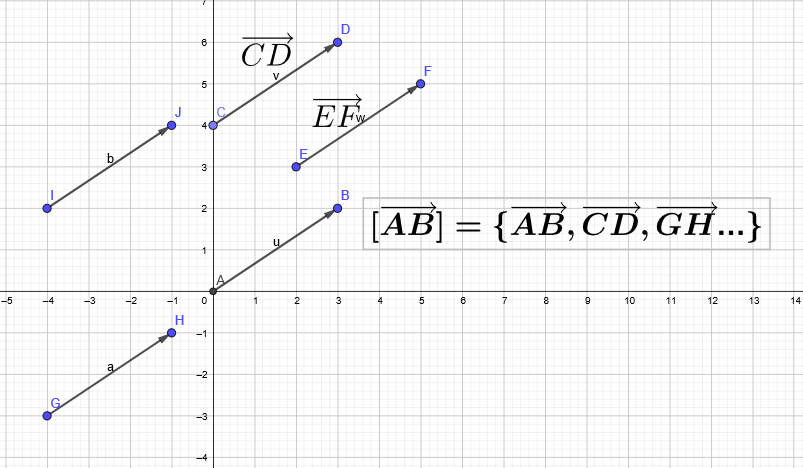
\includegraphics[width=0.9\textwidth]{img/Fijos-libres.png}
    \caption{Los diferentes vectores fijos de $V^2$ que tienen las mismas coordenadas forman parte del vector libre. 
    \newline
    De la misma manera que la idea $\rfrac{1}{2}=\rfrac{2}{4}=\rfrac{3}{6}$ se escribiría formalmente: $\left[\rfrac{1}{2}\right] = \left\{\rfrac{1}{2},\rfrac{2}{4},\rfrac{3}{6} ... \right\}$}
    \label{fig:plano}
\end{figure}


Denotaremos por $[\vec{AB}]$ al vector libre cuyas coordenadas son las del vector que va de $A$ a $B$.

Denotaremos por $\vec{AB}$ al vector fijo que va de $A$ a $B$.





\begin{defn}[Vector\IS definido por dos puntos]
(Página 278)

Dados dos puntos $A=(a_1,a_2,a_3)$ y $B = (b_1,b_2,b_3)$, tenemos 
    \begin{itemize}
        \item $\vec{AB} = \hide{(b_1-a_1, b_2-a_2, b_3-a_3)}$
        \item $\vec{BA} = \hide{(a_1-b_1, a_2-b_2, a_3-b_3)}$ 
    \end{itemize}
\end{defn}

\begin{proof}
Lo único que tenemos para trabajar son vectores de posición. 
%
En este caso son $\vec{a} = \vec{OA}$ y $\vec{b} = \vec{OB}$. 

Tenemos que $\vec{a} + \vec{AB} = \vec{b} \dimplies \vec{AB} = \vec{b}-\vec{a}$.
\end{proof}

\begin{example}
    Halla un vector definido por $A(1,0,3)$ y $B(2,1,2)$.
    
    \hide{\[\vec{AB} = (2-1, 1-0, 2-3) = (1,1,-1)\]}

    \obs Fíjate bien, por favor, que la operación realizada \textbf{no} es una resta de puntos.
\end{example}

\begin{problem}

Utilizando vectores de posición, demuestra que el punto medio entre los puntos $A$ y $B$, que llamamos $M_{AB}$, tiene por coordenadas:

\[M_{AB} = \left(\frac{a_1+b_1}{2},\frac{a_2+b_2}{2},\frac{a_3+b_3}{2}\right)\]

\ppart \textbf{Ampliación:} Dados los puntos $A(a_1,a_2,a_3)$ y $B(b_1,b_2,b_3)$, calcula las coordenadas del punto que divide el segmento $AB$ dejando $\rfrac{1}{3}$ de distancia con $A$ y $\rfrac{2}{3}$ de distancia con $B$. \textit{Pista: planteamiento parecido al punto medio.}

\solution

\[
\left\{
\begin{array}{c}
    \vec{AM} + \vec{MB} = \vec{AB}\\
    \vec{AM} = \vec{MB}\\
    \vec{OM} = ?
\end{array}\right\}
 \implies 
  2\vec{AM} = \vec{AB} \dimplies
  \]\[ 
  2\left(\vec{OM} - \vec{OA}\right) = \vec{AB} \dimplies
  2\vec{OM} = \vec{AB} + 2\vec{OA} = 
  \]\[
  2\vec{OM} = \left(
  b_1-a_1,
  b_2-a_2,
  b_3-a_3
  \right) + 
  \left(
  2a_1 - 0,
  2a_2 - 0,
  2a_3 - 0
  \right) = 
  \left(
  b_1+a_1,
  b_2+a_2,
  b_3+a_3
  \right)\]\[
  \vec{OM} = \left(
  \frac{b_1+a_1}{2},
  \frac{b_2+a_2}{2},
  \frac{b_3+a_3}{2}
  \right)
\]

\end{problem}

% \begin{problem}

% Dado el punto definido por el vector de posición $\vec{OP} = (1,1,1)$ en el sistema de referencia $\{(1,0,0), \mathcal{B} = \{u_1 = (1,0,1), u_2 = (0,2,1), u_3 = (0,0,4)\}\}$, expresa sus coordenadas en el sistema de referencia: 
% %
% $\{(1,1,0), \mathcal{B} = \{\vec{i},\vec{j},\vec{k}\}\}$

% \solution

% ¿Qué significa $\vec{OP} = (1,-2,3)$? Las coordenadas son los coeficientes de los vectores de la base, por lo tanto:

% \[
% P = (1,0,0) + 1·u_1 - 2·u_2+ 3·u_3  \dimplies (1,0,0) + 1·(1,0,1) - 2·(0,2,1)  + 3·(0,0,4) = (2,-4,11)
% \]

% Expresamos el vector $(2,-4,11)$ en el sistema de referencia pedido:

% $(2,-4,11) = (1,1,0) + \lambda_1\vec{i}+ \lambda_2\vec{j}+ \lambda_3\vec{k} \implies (\lambda_1,\lambda_2,\lambda_3) = (1,4,11)$

% \end{problem}

\begin{problem}

Dado el punto definido por el vector de posición $\vec{OP} = (1,1,1)$ en el sistema de referencia $S_1 = \{O_1(1,0,0), \mathcal{B} = \{u_1 = (1,0,1), u_2 = (0,2,1), u_3 = (0,0,4)\}\}$, expresa sus coordenadas en el sistema de referencia: 
%
$S_2=\{O_2(1,1,0), \mathcal{B} = \{\vec{i},\vec{j},\vec{k}\}\}$

\solution

En realidad $\vec{OP} = \vec{O_1P}$, por estar expresado en ese sistema de referencia. 

Entendemos que $O_1(1,0,0)$ no está expresado en función de la base de $S_1$.

¿Qué significa $\vec{O_1P} = (1,1,1)$? Las coordenadas son los coeficientes de los vectores de la base, por lo tanto, tomando $O(0,0,0)$ tenemos:

\[
\vec{OP} = \vec{OO_1} + \vec{O_1P} = (1,0,0) + 1·u_1 + 1·u_2+ 1·u_3  \dimplies\]
\[ (1,0,0) + 1·(1,0,1) +1 ·(0,2,1)  + 1·(0,0,4) = (2,2,6)
\]

Expresamos el vector $\vec{OP}=(2,2,6)$ en el sistema de referencia pedido:
\[\vec{OP} = (2,2,6) = (1,1,0) + \lambda_1\vec{i}+ \lambda_2\vec{j}+ \lambda_3\vec{k} \implies (\lambda_1,\lambda_2,\lambda_3) = (1,1,6) = \vec{O_2P}\]

\vspace{-0.3cm}
\paragraph{Plan b:} 
\[\vec{OP} = \vec{OO_2} + \vec{O_2P} \dimplies \vec{O_2P} = \vec{OP} - \vec{OO_2} = \underbrace{(2,2,6)}_{\ast} - \underbrace{(1,1,0)}_{\Delta} = (1,1,6)\]
\obs Para este planteamiento es \textbf{necesario} que los vectores que operamos (en este caso $\ast$ y $\Delta$) en coordenadas estén expresados en la \textbf{misma base}. 
%
En este caso, dicha base es la base canónica.

\vspace{-0.3cm}
\paragraph{Plan c: } No es necesario pasar por el origen $O(0,0,0)$, aunque pueda resultar más fácil de interpretar así. 

Podríamos haber empezado desde el principio haciendo un razonamiento parecido al plan b. Buscamos $\vec{O_2P}$ y sabemos $\vec{O_1P}$, por lo que podemos plantear:

\[
  \vec{O_1O_2} + \vec{O_2P} = \vec{O_1P} \dimplies \vec{O_2P} = \vec{O_1P} - \vec{O_1O_2}
\]

Como para poder hacer operaciones de vectores en coordenadas necesitamos la misma base, tenemos:

\[
  \vec{O_2P} = \vec{O_1P} - \vec{O_1O_2} = (\textcolor{red}{1},\textcolor{blue}{1},\textcolor{green}{1})_{S_1} - (0,1,0)_{SH} = (\textcolor{red}{1}\vec{u_1} + \textcolor{blue}{1}\vec{u_2} + \textcolor{green}{1}\vec{u_3}) - (0,1,0)
\]\[
  = 1·(1,0,1) +1 ·(0,2,1)  + 1·(0,0,4) - (0,1,0) = (1,1,6)
\]

\begin{itemize}
   \item $(0,1,0)_{SH}$ quiere decir "el vector $(0,1,0)$ expresado en el sistema de referencia habitual".
   \item $(1,1,1)_{S_1}$ quiere decir "el vector $(1,1,1)$ expresado en el sistema de referencia $S_1$".
 \end{itemize} 
\end{problem}


\subsection{La recta}

\obs Dado que la única manera que tenemos de determinar los puntos es a través de vectores de posición, utilizaremos $\vec{p} = (x,y,z)$ de forma equivalente a $[\vec{OP}]$ para referirnos a un punto cualquiera del espacio, al que accedemos a través de su vector de posición.

Formas de determinar una recta:
\begin{enumerate}
  \item Un punto\footnote{O su vector de posición} y un vector director.
  \subitem 2 puntos (se reduce al caso anterior)
  \subitem Un punto y una condición de paralelismo (se reduce al primer caso)
  \item 2 planos secantes.
  \item Un punto y un plano perpendicular (se verá en geometría euclídea).
\end{enumerate}

Como todo con lo que vamos a trabajar son operaciones con vectores con coordenadas en un sistema de referencia, en realidad el punto de origen del sistema de referencia no es relevante. (Ver ejemplo \ref{example::origen_ref}).

\subsubsection{Ecuaciones de la recta}

La 
%
\concept[Ecuación de la recta\IS vectorial]{ecuación vectorial de la recta} $r$ determinada por el punto $A$, cuyo vector de posición es $\vec{a}$, con vector director $\vec{u_r} $  es $r : \vec{p} = \vec{a} + \lambda \vec{u_r}$, con $\lambda\in\real, \forall P\in\real$ (ver \fref{fig::recta_ecuacion_vectorial})
%
De esta manera quedan determinados los vectores de posición de todos los puntos de la recta $r$.


\begin{figure}[hptb]
    \centering
    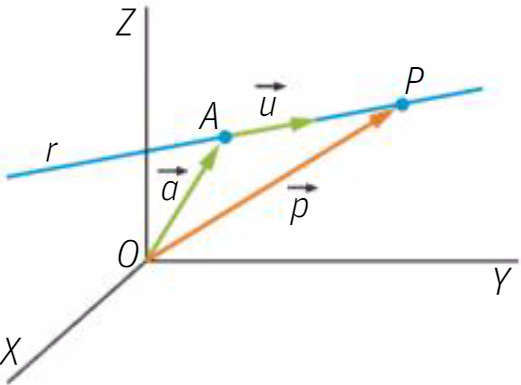
\includegraphics[width=0.4\textwidth]{img/EcVectorialRecta.png}
    \caption{Representación gráfica de la ecuación vectorial de la recta.}
    \label{fig::recta_ecuacion_vectorial}
\end{figure}


¿Es posible construir la recta sin ese parámetro $\lambda$? En realidad,
$$\underbrace{r : \vec{p} = \vec{a} + \lambda \vec{u_r}}_{(0)}\dimplies \underbrace{r:\displaystyle \left\{
\begin{array}{c} 
  x = a_1 + \lambda u_1\\
  y = a_2 + \lambda u_2 \\ 
  z = a_3 + \lambda u_3
\end{array}\right\}}_{(1)} \implies \underbrace{r:\frac{x-a_1}{u_1} = \frac{y-a_2}{u_2} = \frac{z-a_3}{u_3}}_{(2)}$$

\begin{itemize}
    \item A $(1)$ lo denominamos \concept[Ecuación de la recta\IS paramétrica]{ecuación paramétrica de la recta}
    \item A $(2)$ lo denominamos \concept[Ecuación de la recta\IS continua]{ecuación continua de la recta}
\end{itemize}

\[
\frac{x-a_1}{u_1} = \frac{y-a_2}{u_2} = \frac{z-a_3}{u_3}\overset{(1)}{\implies} \left\{
\begin{array}{c}
     \displaystyle\frac{x-a_1}{u_1} = \frac{y-a_2}{u_2}\\
     \displaystyle\frac{y-a_2}{u_2} = \frac{z-a_3}{u_3}
\end{array}\right\} \implies
\underbrace{\left\{\begin{array}{cccc}
     Ax + &By    &     & = D\\
          &B'y   &+ C'z  & = D
\end{array}\right\}}_{(2)}
\]



Donde:
\begin{itemize}
    \item (1) \hide{Se han elegido estas 2 parejas, pero podrían haberse elegido otras, dando lugar a otras ecuaciones implícitas de la misma recta.}
    \item (2) \hide{\concept[Ecuación de la recta\IS implícita]{ecuación implícita de la recta}}
    \subitem \obs \hide{Si interpretáramos las ecuaciones implícitas de la recta como un sistema de ecuaciones, tendríamos un sistema compatible indeterminado con grado de libertad 1.}
    \subitem \obs La dimensión de la recta es 1. \emph{¿Como el grado de indeterminación? Guau...}
\end{itemize}

\begin{problem}
    \ppart 
    Halla todas las ecuaciones de la recta que pasa por $A(0,1,2)$ y es paralela a la que pasa por $B(1,-2,-1)$ y $C(1,0,0)$
    \ppart 
    Halla un vector director de la recta $r:\displaystyle\frac{x-2}{1} = \frac{y-3}{5} = \frac{z-1}{4}$
    \ppart 
    Halla un vector director de la recta $r:\displaystyle\left\{\begin{array}{c} 2x+3y=4\\2x-y+3z=0\end{array}\right\}$
    \solution

\end{problem}

\textbf{Deberes:} 
\begin{itemize}
  \item Página 279.13,14.
  \item Página 281.18-21.
\end{itemize}

\subsection{El plano}

\subsubsection{Ecuaciones del plano}

Un plano queda determinado por \hide{un punto y dos vectores linealmente independientes}

La 
%
\concept[Ecuación del plano\IS vectorial]{ecuación vectorial del plano} 
%
$\pi$ determinada por el punto $A$ y los vectores linealmente independientes $\vec{V_{\pi}}$ y $\vec{W_{\pi}}$  es $r : \vec{p} = \vec{A} + \lambda \vec{V_{\pi}} + \mu\vec{W_{\pi}}$, con $\lambda\in\real$ (ver ). De esta manera quedan determinados los vectores de posición de todos los puntos del plano.

Como en el caso de la recta, podemos escribir esta ecuación en forma de sistema con parámetros:

$$\pi : \vec{p} = \vec{A} + \lambda \vec{V_{\pi}} + \mu\vec{W_{\pi}}\dimplies \underbrace{\pi:\displaystyle \left\{\begin{array}{c} x = a_1 + \lambda v_1 + \mu w_1\\y = a_2 + \lambda v_2 + \mu w_2 \\ z = a_3 + \lambda v_3 + \mu w_3 \end{array}\right\}}_{(1)} $$

 A $(1)$ lo denominamos \concept[Ecuación del plano\IS paramétrica]{ecuación paramétrica del plano}

\[
\pi:\displaystyle \left\{
\begin{array}{c} 
x - a_1 = \lambda v_1 + \mu w_1\\
y - a_2 = \lambda v_2 + \mu w_2 \\ 
z - a_3 = \lambda v_3 + \mu w_3 
\end{array}\right\}
\]
Como los vectores $\vec{v},\vec{w}$ son linealmente independientes y el vector $AX$ es una combinación lineal de los otros 2 (ver \ref{fig:plano}), tenemos:

\[
\left|
\begin{array}{ccc} 
x - a_1 & v_1 & w_1\\
y - a_2 & v_2 & w_2 \\ 
z - a_3 & v_3 & w_3 
\end{array}\right| = 0
\]

Desarrollando esta ecuación, tendríamos una ecuación del tipo $Ax+By+Cz + D = 0$, que llamamos \concept[Ecuación del plano\IS implícita]{Ecuación implícita del plano}.


\begin{figure}[hptb]
    \centering
    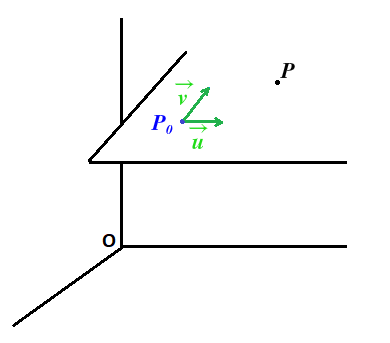
\includegraphics[width=0.65\textwidth]{img/ecplanos.png}
    \caption{Plano generado por un punto y dos vectores}
    \label{fig:plano}
\end{figure}

\begin{problem}
    \textbf{Calcula las ecuaciones del plano que pasa por los puntos $A(1,1,1), B(2,2,2), C(1,2,3)$}

    \solution 

    \hide{
    El primer paso sería calcular 2 vectores linealmente independientes de estos 3 puntos, para comprobar que los 3 puntos forman un plano (y no una recta).

    $\vec{AB} = (1,1,1) \quad\quad \vec{AC} = (0,1,2)$, que son linealmente independientes al no ser proporcionales.

    Ecuación vectorial: $\pi: \vec{p} = (1,1,1) + \mu\vec{AB} + \lambda\vec{AC}, \lambda,\mu\in\real$

    Ecuación paramétrica: $
    \displaystyle\left\{ \begin{array}{c}
      x = 1 + \mu\\
      y = 1 + \mu + \lambda\\
      z = 1 + \mu + 2\lambda
    \end{array} \right\}\text{ con } \lambda,\mu\in\real$

    Ecuación implícita: 

    \[
      \displaystyle \begin{vmatrix}
      x - 1 & 1 & 0\\
      y - 1 & 1 & 1\\
      z - 1 & 1 & 2\\
    \end{vmatrix} = 0 \dimplies \cdots \dimplies x - 2y+z=0
    \]
    }
\end{problem}


\begin{problem}
\ppart Halla la ecuación de 2 rectas que pertenezcan al mismo plano.
\ppart Halla un vector director del plano: $\pi_1: x+y+z = 3$
\ppart Halla el plano paralelo a $\pi_2: x+y+z = 3$ que pase por el origen de coordenadas.
\ppart Halla el plano paralelo al $XY$ que pasa por $A(-1,2,-2)$.
\obs Llamamos plano $XY$ al plano "del suelo", es decir, al plano $z=0$.

\ppart Página 283, ejercicios 25-28.

\solution

\end{problem}

\subsection{Posiciones relativas}

\subsubsection{Entre 2 planos}  

\begin{framed}
\textbf{Ecuaciones vectoriales o paramétricas:}
  \begin{itemize}
    \item Si 2 planos comparten 3 puntos, entonces son el mismo plano.
    \item Si los 4 vectores directores de los 2 planos son linealmente independientes, entonces los planos son secantes en un punto.
    \item Si la matriz formada por los 4 vectores directores de los 2 planos tiene rango 3, los planos son secantes en una recta.
    \item Si la matriz formada por los 4 vectores directores de los 2 planos tiene rango 2, los planos son paralelos.
    \item Si 2 planos paralelos comparten un punto, entonces son coincidentes.
  \end{itemize}
\end{framed}



\subparagraph{Ecuaciones implícitas}

\[
\left\{\begin{array}{c}
\pi_1: Ax+By+Cz = D\\
\pi_2: A'x+B'y+C'z = D'
\end{array}\right\}
\]

Obtenemos las matrices: $M = \displaystyle\begin{pmatrix}A&B&C\\A'&B'&C'\end{pmatrix}$ y $M^* = \displaystyle\begin{pmatrix}A&B&C&D\\A'&B'&C'&D'\end{pmatrix}$

\begin{framed}
  \begin{itemize}
    \item $Rg(M) = Rg(M^*) = 1 $\hide{ coincidentes.}
    \item $Rg(M) < Rg(M^*) = 2 $\hide{ paralelos.}
    \item $Rg(M) = Rg(M^*) = 2 $\hide{ secantes.}
  \end{itemize}
\obs En realidad, sería como las ecuaciones implícitas de la recta.
\end{framed}

\subsubsection{Entre 3 planos}

\subparagraph{Ecuaciones vectorial o paramétricas}

Se pasa a implícitas.

\subparagraph{Ecuaciones implícitas}
\[
\left\{\begin{array}{c}
\pi_1: Ax+By+Cz = D\\
\pi_2: A'x+B'y+C'z = D'\\
\pi_3: A''x+B''y+C''z = D''\\
\end{array}\right\}
\]

Obtenemos las matrices: 
$M  = \displaystyle\begin{pmatrix}
A&B&C\\
A'&B'&C'\\
A''&B''&C''
\end{pmatrix}
$ y 
$M^* = \displaystyle\begin{pmatrix}
A&B&C&D\\
A'&B'&C'&D'\\
A''&B''&C''&D''
\end{pmatrix}
$

Las posibilidades son: (ver figura \ref{fig:PosicionesRelativasPlanos})
\begin{framed}
  \begin{itemize}
    \item $Rg(M) = Rg(M^*) = 1 $\hide{ SCI, secantes en un plano [grado de indeterminación 2, por lo que hay dos parámetros. \textbf{Coincidentes}.}
    \item $Rg(M) < Rg(M^*) = 2 $\hide{ paralelos.}
    \item $Rg(M) = Rg(M^*) = 2 $\hide{ SCI, secantes en una recta [grado de indeterminación 1, por lo que hay un parámetro.}
    \item $Rg(M) = 2 < Rg(M^*) = 3 $\hide{ no se cortan los 3. Sistema incompatible}
    \item $Rg(M) = Rg(M^*) = 3 $\hide{ SCD, secantes en un punto que es la solución del sistema.}
  \end{itemize}  
\end{framed}

\begin{figure}[hptb]
    \centering
    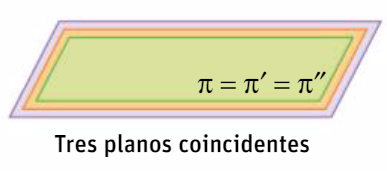
\includegraphics[width=0.65\textwidth]{img/Captura1.png}
    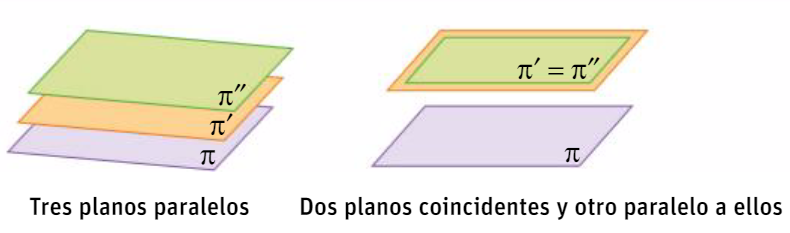
\includegraphics[width=0.95\textwidth]{img/Captura2.png}
    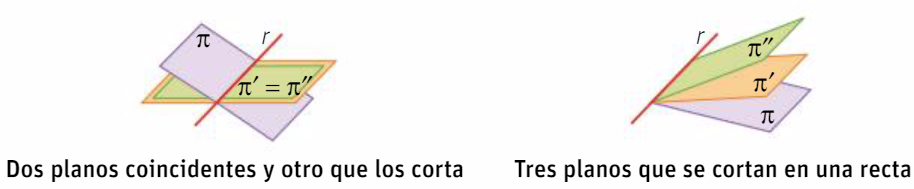
\includegraphics[width=1.1\textwidth]{img/Captura3.png}
    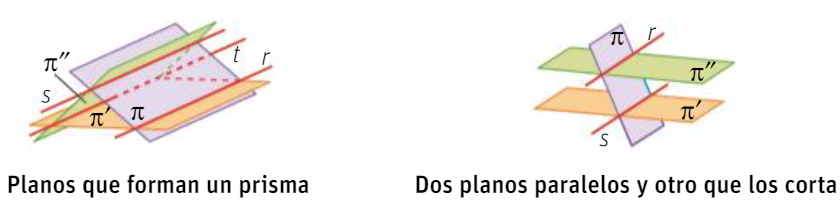
\includegraphics[width=1.1\textwidth]{img/Captura4.png}
    \caption{Representación gráfica de las posiciones relativas de 3 planos.}
    \label{fig:PosicionesRelativasPlanos}
\end{figure}




\subsection{Posiciones relativas entre recta y plano}

\paragraph{Ecuaciones implícitas: } si tanto la recta como el plano están dados en ecuaciones implícitas, estaríamos en la posición relativa de 3 planos, sabiendo que 2 de ellos son secantes en una recta.

\paragraph{Ecuaciones paramétrica: } $\pi: \{P_{\pi},\vec{v_{\pi}}, \vec{w_{\pi}}\}$ 

\begin{center}
\begin{tabular}{ccc}
$P_r \in \pi $ & $\vec{v_r}$ LD de $v_{\pi}, \vec{w}_{\pi}$ & \textbf{Conclusión}\\\hline
No & No & Secantes en un punto\\
No & Sí & Recta paralela\\
Sí & No & Secantes en un punto\\
Sí & Sí & Recta contenida en el plano\\
\end{tabular}
\end{center}

\paragraph{Plano implícito, recta paramétrica: } comprobamos si existe algún valor de $\lambda_{r}$ para el que se cumpla la ecuación implícita del plano. 
\begin{itemize}
  \item $\exists!\lambda \implies $ secante.
  \item $\lambda \in \real \implies$ contenida.
  \item $\not\exists \lambda \implies $ paralela.
\end{itemize}

Deberes: Hoja resumen de teoría,105ab,107ab

\subsubsection{Posiciones relativas entre 2 rectas:}

Dadas las rectas 
$r:\vec{p} = \vec{a} + \lambda\vec{u},\quad \lambda\in\real$
y
$s:\vec{p} = \vec{b} + \lambda\vec{w},\quad \lambda\in\real$. 

Si los vectores directores son paralelos (proporcionales), las rectas pueden ser paralelas o coincidentes. 
%
Para poder distinguir , podríamos ver si un vector formado por un punto de cada recta es también proporcional (entonces serían coincidentes) o si no (entonces serían secantes).

De la misma manera, si los vectores son linealmente independientes las rectas pueden cruzarse o cortarse. 
%
Para distinguir estos 2 casos, podríamos ver si un vector formado por un punto de cada recta es linealmente dependiente a los otros 2 (entonces serían secantes porque formarían un plano que contiene al vector) o si no (entonces se cortarían en el espacio).

Así, buscamos estudiar la dependencia lineal de los 2 vectores directores ($\vec{u},\vec{w}$) y de los 2 vectores directores respecto de un vector formado, arbitrariamente, con 2 puntos de las rectas ($\vec{AB}$, con $A(a_1,a_2,a_3)\in r$ y $B(b_1,b_2,b_3)\in s$). 
%
Para ello, formamos las matrices:

$M  = \displaystyle\begin{pmatrix}
u_1&w_1\\
u_2&w_2\\
u_3&w_3
\end{pmatrix}
$ y 
$M^* = \displaystyle\begin{pmatrix}
u_1&w_1&b_1-a_1\\
u_2&w_2&b_2-a_2\\
u_3&w_3&b_3-a_3\\
\end{pmatrix}
$

\begin{framed}
  \begin{itemize}
    \item $Rg(M) = Rg(M^*) = 1 $\hide{ SCI, secantes en una recta [grado de indeterminación 1, por lo que hay dos parámetros. \textbf{Coincidentes}.]}
    \item $Rg(M) = 1 < Rg(M^*) = 2 $\hide{ paralelas.} 
    \item $Rg(M) = Rg(M^*) = 2 $\hide{ SCI, secantes en un plano [dimensión 2]. $\vec{AB}$ se puede escribir como combinación lineal de $\vec{u}$ y $\vec{w}$}
    \item $Rg(M) = 2 < Rg(M^*) = 3 $\hide{ se cruzan en el espacio.} 
  \end{itemize}  
\end{framed}
\obs También se podría trabajar con las matrices traspuestas si uno está más familiarizado con estudiar el rango como combinaciones lineales de filas en lugar de columnas.

\begin{problem}
Página 289, ejercicios 52, calculando puntos de cortes
\solution

\end{problem}


\subsubsection{Haz (no se pide en selectividad, así que se salta)}
\paragraph{Haz de rectas paralelas: } cambia el punto, manteniendo fijo el vector. 
\paragraph{Haz de rectas secantes: } cambia el vector (sin ser nunca nulo), mantiene fijo el punto.
\paragraph{Haz de planos paralelelos: } cambia el punto, mantiene los vectores
\paragraph{Haz de planos secantes en una recta: } mantiene un vector y un punto, cambia el otro vector.

\begin{problem}
Tema 11: 56,57,59,60.
\solution
\end{problem}

Deberes: 118,136,143

\subsubsection{Practicamos en general}

Tema 11: 
122,127,130,134,135,136,139,140,143,145,149,150

Tema 11:
\begin{itemize}
  \item Básicos: 83,91,92,93a,98,100,101a,103a,104a,105,106,107d,108
  \item Síntesis: 111-119
  \item Completos: 122-124,127,129-133
\end{itemize}





\section{Geometría euclídea}

Llamamos geometría euclídea al espacio en el que podemos medir, cosa que hasta ahora no era posible.

Todo surge desde el módulo de un vector. Llamamos \concept[Módulo de un vector]{módulo de un vector} a la longitud que tiene. Dado $\vec{v}$, se define el módulo como $|\vec{v}|$.

Si el vector $\vec{v}$ tiene como coordenadas $\vec{v} = (v_1,v_2,v_3)$ en la base canónica, podemos calcular su módulo como $|\vec{v}| = \sqrt{v_1^2+v_2^2+v_3^2}$

\begin{prop}
$\left|\lambda\vec{v}\right| = |\lambda|·|\vec{v}|$
\end{prop}
\begin{proof}
$$|\lambda·\vec{v}| = \sqrt{(\lambda·v_1)^2+(\lambda·v_2)^2+(\lambda·v_3)^2} = \sqrt{\lambda^2 (v_1^2+v_2^2+v_3^2)} = |\lambda| ·\left|\vec{u}\right|$$
\end{proof}

\begin{defn}[Vector\IS unitario]
\[\vec{u}\in V^3 \text{ es unitario } \dimplies \left|\vec{u}\right|=1\]
\end{defn}

\begin{problem}
Dado el vector $\vec{u} = (0,3,4)$, encuentra:
\ppart Un vector unitario con la misma dirección. ¿Cuántos hay?
\ppart Un vector unitario con la misma dirección y el mismo sentido. ¿Cuántos hay?
\solution

Calculamos $\vec{u} = \sqrt{0^2+3^2+4^5} = \sqrt{25} = 5$

\spart Buscamos $\vec{v} = (0,3\lambda,4\lambda)$ tal que $|\vec{v}| = 1$

\[|\vec{v}| = \sqrt{0^2+(3\lambda)^2+(4\lambda)^2} = \sqrt{25\lambda^2} =1 \dimplies \lambda=\pm\rfrac{1}{5}\]

Hay dos vectores unitarios ocn la misma dirección: $\vec{v_1} = \left(0,\rfrac{3}{5},\rfrac{4}{5}\right)$ y $\vec{v_2} = \left(0,-\rfrac{3}{5},-\rfrac{4}{5}\right)$

Hay 2 vectores unitarios con la misma dirección.

\obs Estos dos vectores tienen la misma dirección pero sentido contrario.

\spart El único vector unitario con la misma dirección y el mismo sentido es $\vec{v_2}$

\end{problem}

\obs ¿Es casualidad que $\lambda = \rfrac{1}{\left|\vec{u}\right|}$?  

\begin{prop}
Dado $\vec{u} = (u_1,u_2,u_3)$
\[\text{El vector } \frac{1}{\left|\vec{u}\right|}\vec{u} = \left(\frac{u_1}{\left|\vec{u}\right|},\frac{u_2}{\left|\vec{u}\right|},\frac{u_3}{\left|\vec{u}\right|}\right)\text{ es unitario}\]
\end{prop}

\begin{proof}
Para demostrarlo solamente es necesario aplicar la propiedad del módulo: $\left|\lambda·\vec{u}\right| = |\lambda|·\left|\vec{u}\right|$

\[\left|\frac{1}{\left|\vec{u}\right|}\vec{u}\right| = \frac{1}{\left|\vec{u}\right|}\left|\vec{u}\right| = 1\]
\end{proof}

\subsection{Productos (escalar, vectorial y mixto)}

% \paragraph{Introducción sobre el origen del producto escalar y vectorial}

% Fuentes consultadas:
% \begin{itemize}
%   \item \href{http://www.suitcaseofdreams.net/Geometric_multiplication.htm}{Relación forma polar y binómica del producto complejo}
%   \vspace{-0.4cm}
%   \item \href{https://www2.clarku.edu/faculty/djoyce/complex/mult.html}{Interpretación geométrica del producto complejo}
%   \vspace{-0.4cm}
%   \item \href{https://www.quora.com/Who-invented-the-dot-product-and-cross-product}{Historia y aplicación de los cuaterniones los productos}
%   \vspace{-0.4cm}
%   \item \href{https://es.wikipedia.org/wiki/Cuaterni%C3%B3n}{ Extensión de los complejos al grupo de los quaterniones}
% \end{itemize}

% Dados 2 números complejos $z_1 = a_1+b_1i$, $z_2 = a_2+b_2i$. Expresando estos números complejos en forma polar tenemos: $z_1=r_{\alpha_1}$ y $z_2 = s_{\alpha_2}$.  

% $z_1·z_2 = (a_1a_2 - b_1b_2) + (a_1b_2+a_2b_1)i = r·s_{\alpha_1+\alpha_2}$.

% Tomando $z_1·\bar{z_2} = (a_1a_2 + b_1b_2) + (a_1b_2-a_2b_1)i = r·s_{\alpha_1-\alpha_2}
% $

% \subparagraph{Estudio de la parte real (producto escalar)}

% En $Re(z_1·\bar{z_2}) = a_1a_2 + b_1b_2 = Re(r·s_{\alpha_1-\alpha_2})$

% Para calcular $Re(r·s_{\alpha_1-\alpha_2}) = Re(r·s·\cos(\alpha_1-\alpha_2) + i·r·s·\sen(\alpha_1-\alpha_2)$, por lo que podemos completar:

% $ a_1a_2 + b_1b_2 = |z_1\;||\;z_2|·\cos(\alpha_1-\alpha_2)$, y, siendo conscientes que $\alpha_1-\alpha_2$ es el ángulo que forman los 2 vectores, obtenemos la expresión del producto escalar de 2 vectores.


% \subparagraph{Estudio de la parte imaginaria (producto vectorial)}

% Al extender este razonamiento al grupo de los cuaterniones, tendríamos:

% \newcommand{\quat}{\vec}

% $Re(z_1\bar{z_2}) = Re\left((b_1\quat{i}+c_1\quat{j}+d_1\quat{k})·(-b_2\quat{i}-c_2\quat{j}-d_2\quat{k})\right) = (b_1b_2+c_1c_2+d_1d_2)$

% Lo espectacular viene al considerar la parte "imaginaria" (aunque no tengamos claro cómo se define ese concepto en los cuaterniones):

% $Im(z_1\bar{z_2}) = f(\quat{i},\quat{j},\quat{k})$, cuya expresión analítica es la del producto vectorial, ya que en grupo de los cuaterniones $\quat{i}\quat{j}=\quat{k}$ y todo eso.

\subsubsection{Producto escalar}

\begin{defn}[Producto\IS escalar]

Dados $\vec{v},\vec{w}$, se define $\appl{\cdot}{V^3\times V^3}{\real}$ como 
\[\vec{v}·\vec{w} = |\vec{w}|·|\vec{v}|\cdot\cos\left(\widehat{\vec{v},\vec{w}}\right)\]
\end{defn}

\paragraph{Propiedades:} $\forall\vx,\vx,\vz\in V^3$

\begin{itemize}
  \item \textbf{Conmutativo: } $\vx·\vy = \vy·\vx$
  \item \textbf{Bilineal:}
  \subitem  $(λ\vx)·\vy=λ(\vx·\vy)$
  \subitem  $\vx·(\vy+\vz) = \vx·\vy + \vx·\vz$
  \item \textbf{No negatividad:} $\vx·\vx ≥0$
\end{itemize}


¿Qué ocurre si no cooncemos el ángulo que forman los 2 vectores? Necesitamos otra manera de calcular el producto escalar. 

\begin{prop}[Expresión analítica del producto\IS escalar]

Dados $\vec{v}=(v_1,v_2,v_3),\vec{w}=(w_1,w_2,w_3)\in V^2$ respecto de la base canónica $\mathcal{B} = \{\vi,\vj,\vk\}$, entonces $\vec{v}·\vec{w} = v_1·w_1 + v_2·w_2+ v_3·w_3$
\end{prop}

\begin{proof}

\[
\vec{v}·\vec{w} = \left(v_1\vi+v_2\vj+v_3\vk\right)·\left(w_1\vi+w_2\vj+w_3\vk\right)\]
\[
v_1w_1\vi\vi+v_1w_2\vi\vj+v_1w_3\vi\vz+\]\[
v_2w_1\vj\vi+v_2w_2\vj\vj+v_2w_3\vj\vz+\]\[
v_3w_1\vz\vi+v_3w_2\vz\vj+v_3w_3\vz\vz = 
\]
\[
v_1w_1+v_1w_2·0+v_1w_3·0+\]\[
v_2w_1·0+v_2w_2+v_2w_3·0+\]\[
v_3w_1·0+v_3w_2·0+v_3w_3= \]
\[v_1·w_1 + v_2·w_2 + w_3·v_3\]
\end{proof}


\begin{prop} 
\[
\vec{u}·\vec{u} = \left|\vec{u}\right|^2
\]
\end{prop}


\begin{defn}[Ortogonalidad y perpendicularidad]

Decimos que $\vec{u},\vec{v}\in V^3$ son \textbf{perpendiculares} si forman un ángulo recto. Escribiremos $\vec{u}\perp\vec{v}$.

Decimos que $\vec{u},\vec{v}\in V^3$ son \textbf{ortogonales} si $\vec{u}·\vec{v} = 0$
\end{defn}

\obs Hay ligero matiz. Fíjate que $\vec{u}\perp\vec{v} \implies \vec{u}·\vec{v} = 0$ pero no al revés, ya que $\vec{0} = (0,0)$ es ortogonal a todos pero perpendicular a ninguno.

\paragraph{Clasificación de bases de vectores}

Dada la base $\mathcal{B} = \left\{\vec{a},\vec{b},\vec{c}\right\}$.

\begin{itemize}
  \item Decimos que es una base \concept[Base\IS ortogonal]{ortogonal} si y solo si $\vec{a}\perp\vec{b}\perp\vec{c}$.
  \item Decimos que es una base \concept[Base\IS ortonormal]{ortonormal} si y solo si es una base ortogonal y $|\vec{a}| = |\vec{b}| = |\vec{c}|$
\end{itemize}


\obs Con el producto escalar podemos calcular el \concept[Angulo entre\IS vectores]{angulo que forman 2 vectores}. Dado que $\vec{u}·\vec{v} = \left|\vec{u}\right|·\left|\vec{u}\right|·\cos\left(\widehat{\vec{u},\vec{v}}\right)$, podemos despejar 

\[\cos\left(\widehat{\vec{u},\vec{v}}\right) = \frac{\vec{u}·\vec{v}}{\left|\vec{u}\right|·\left|\vec{u}\right|}\]


\begin{problem}

Halla el ángulo que forman los vectores $\vec{u}=\left(2,-3,1\right),\vec{v}=\left(1,2,-2\right)$


\solution


\[\cos\left(\widehat{\vec{u},\vec{v}}\right) = \frac{\vec{u}·\vec{v}}{\left|\vec{u}\right|·\left|\vec{u}\right|} = \frac{2·1-3·2+1·(-2)}{\sqrt{14}{\sqrt{9}}} = \frac{-2}{\sqrt{14}}\]

Para calcular el ángulo que forman: 

\[
\widehat{\vec{u},\vec{v}} = \arccos \frac{-2}{\sqrt{14}} = 122º 19'
\]
\end{problem}

\begin{problem}

Halla el valor de $k$ para que el ángulo que forman los vectores $\vec{a} = (1,k,k)$ y $\vec{b} = (1,-2,1)$ sea de 60º. 
\solution
$k=-\rfrac{1}{2}$

\end{problem}

\paragraph{Interpretación geométrica del producto escalar}

\hl{Por terminar}

\subsubsection{Producto vectorial}


\begin{defn}[Producto\IS vectorial]
Dados $\vec{v},\vec{w}$, se define $\appl{\times}{V^3\times V^3}{V^3}$ como 
\[\vec{v}\times\vec{w} = |\vec{w}|·|\vec{v}|\cdot\sen\left(\widehat{\vec{v},\vec{w}}\right)·\vec{n}\]

donde $\vec{n}$ es un vector unitario y ortogonal a $\vec{v},\vec{w}$ y su sentido está dado por la regla de la \textit{mano derecha}.
\end{defn}

\paragraph{Propiedades:} $\forall\vx,\vx,\vz\in V^3$

\begin{itemize}
  \item \textbf{Anticonmutativo: } $\vx\times\vy = -\vy\times\vx$ 
  \subitem Al alterar el orden del producto, el sentido del vector resultante es contrario.
  \item \textbf{Homogénea:} $(λ\vx)\times\vy=λ(\vx\times\vy)$
  \item\textbf{Distributiva:}  $\vx\times(\vy+\vz) = \vx\times\vy + \vx\times\vz$
  \item $\vx\times\vx=0$
  \subitem Dados dos vectores $\vv\neq0$ y $\vw \vv\times\vw = 0 \dimplies \vv\;||\;\vw$
\end{itemize}

\begin{prop}[Expresión analítica del producto\IS vectorial]

Dados $\vec{v}=(v_1,v_2,v_3),\vec{w}=(w_1,w_2,w_3)\in V^2$ respecto de la base canónica $\mathcal{B} = \{\vi,\vj,\vk\}$, entonces 
\[\vec{v}\times\vec{w} = \left|\begin{matrix}\vec{i}&\vec{j}&\vec{k}\\v_1&v_2&v_3\\w_1&w_2&w_3\end{matrix}\right|\]
\end{prop}

\begin{proof}

Para la demostración es necesario tener en cuenta que: $\vi\times\vj=\vk$, $\vj\times\vk=\vi$, $\vk\times\vi=\vj$

\[
\vec{v}\times\vec{w} = \left(v_1\vi+v_2\vj+v_3\vk\right)\times\left(w_1\vi+w_2\vj+w_3\vk\right)\]
\[
v_1w_1\vi\times\vi+v_1w_2\vi\times\vj+v_1w_3\vi\times\vz+\]\[
v_2w_1\vj\times\vi+v_2w_2\vj\times\vj+v_2w_3\vj\times\vz+\]\[
v_3w_1\vz\times\vi+v_3w_2\vz\times\vj+v_3w_3\vz\times\vz=
\]
\[
v_1w_2\vk-v_1w_3\vj-v_2w_1\vk+v_2w_3\vi+v_3w_1\vj-v_3w_2\vi = \]\[
(v_2w_3-w_2v_3)\vi -(v_1w_3-w_3v_1)\vj+ (v_1w_2-w_2v_1)\vk = 
\]
\[
\left|\begin{matrix}v_2&v_3\\w_2w_3\end{matrix}\right|\vi - 
\left|\begin{matrix}v_1&v_3\\w_1w_3\end{matrix}\right|\vj +
\left|\begin{matrix}v_1&v_2\\w_1w_2\end{matrix}\right|\vk = \left|\begin{matrix}\vec{i}&\vec{j}&\vec{k}\\v_1&v_2&v_3\\w_1&w_2&w_3\end{matrix}\right|
\]
\end{proof}


\begin{example}
Dados $\vec{u}=(-1,3,-3)$ y $\vec{v} = (3,-2,0)$
\[
\vec{u}\times\vec{v} = \crossprod{-1}{3}{-3}{3}{-2}{0} =\crossprodcalc{-1}{3}{-3}{3}{-2}{0}
\]
\end{example}

\paragraph{Interpretación geométrica del producto vectorial}

\hl{Por terminar}

\subsubsection{Producto mixto}
\begin{defn}[Producto\IS mixto]
Dados $\vec{u},\vec{v},\vec{w}$, se define $\appl{\times}{V^3\times V^3\times V^3}{\real}$ como 
\[\left[\vec{u},\vec{v},\vec{w}\right] = \vec{u}·\left(\vec{v}\times\vec{w}\right)\]
\end{defn}

\paragraph{Propiedades:} $\forall\vx,\vx,\vz\in V^3,a,b,c\in\real$

\begin{itemize}
  \item $[\vx,\vy,\vz]=[\vz,\vx,\vy]=[\vy,\vz,\vx]$ 
  \item $[\vx,\vy,\vz]=-[\vx,\vz,\vy]$ 
  \subitem De la misma manera, también se cumplen: $[\vx,\vy,\vz]=-[\vy,\vx,\vz]\quad$ y $\quad[\vx,\vy,\vz]=-[\vz,\vy,\vx]$
  \item $[a\vx,b\vy,c\vz]=abc[\vz,\vx,\vy]$ 
  \item $[\vx,\vy,\vz]=0 \dimplies \vx,\vy,\vz$ son linealmente dependientes.
\end{itemize}

\begin{prop}[Expresión analítica del producto\IS vectorial]

Dados $\vec{u}=(u_1,u_2,u_3),\vec{v}=(v_1,v_2,v_3),\vec{w}=(w_1,w_2,w_3)\in V^3$ respecto de la base canónica $\mathcal{B} = \{\vi,\vj,\vk\}$, entonces 
\[[\vu,\vv,\vw] = \vu·(\vec{v}\times\vec{w}) = \detwrite{u_1}{u_2}{u_3}{v_1}{v_2}{v_3}{w_1}{w_2}{w_3}\]
\end{prop}

\begin{proof}

Para la demostración es necesario tener en cuenta que: $\vi\times\vj=\vk$, $\vj\times\vk=\vi$, $\vk\times\vi=\vj$

\[
\vec{u}·(\vec{v}\times\vec{w}) = \left(u_1,u_2,u_3\right)·
\left(\left|\begin{matrix}v_2&v_3\\w_2w_3\end{matrix}\right|,
\left|\begin{matrix}v_1&v_3\\w_1w_3\end{matrix}\right|,
\left|\begin{matrix}v_1&v_2\\w_1w_2\end{matrix}\right|\right) = \left|\begin{matrix}u_1&u_2&u_3\\v_1&v_2&v_3\\w_1&w_2&w_3\end{matrix}\right|
\]
\end{proof}


\begin{example}
Dados $\vec{u} = (-1,2,0),\vec{v} = (-1,-2,2), \vec{w} = (-2,3,-1)$


\[
\left[\vec{u},\vec{v},\vec{w}\right] = \detwrite{-1}{2}{0}{-1}{-2}{2}{-2}{3}{-1} = \detwritecalc{-1}{2}{0}{-1}{-2}{2}{-2}{3}{-1}
\]
\end{example}

\paragraph{Interpretación geométrica del producto mixto:}
\hl{Por terminar}

\obs Acabado tema 9.

\subsection{Aplicación de los productos}

\subsubsection{Vector normal del plano}

\begin{prop}
Dado el plano $\pi:Ax+By+Cz+D=0$, el vector $\vec{n} = (A,B,C)$ es un vector perpendicular (o normal).
\end{prop}

\begin{proof}

Consideramos dos puntos del plano diferentes: $P\in\pi, Q\in\pi$, con $P(p_1,p_2,p_3), Q(q_1,q_2,q_3)$ y $\vec{PQ} = (q_1-p_1,q_2-p_2,q_3-p_3)$

Comprobamos que $ \vec{PQ}·\vec{n} = 0$

\[\vec{PQ}·\vec{n} =  (q_1-p_1,q_2-p_2,q_3-p_3)·(A,B,C) =\]
\[ Aq_1-Ap_1+Bq_2-Bp_2+Cq_3-Dp_3 = Aq_1+Bq_2+Cq_3 - (Ap_1+Bp_2+Cp_3) \overset{(1)}{=} D - D = 0\]

$(1):$ Dado que $P\in\pi$, las coordenadas del punto $P$ cumplen la ecuación del plano.
\end{proof}

\begin{problem}

Construye el plano perpendicular a la recta $r: (x,y,z) = (0,1,3) + \lambda (2,3,1)$ que pasa por $P(0,1,1)$

\solution

Buscamos $\pi\perp r$, por lo que podemos tomar $\vec{n_{\pi}} = \vec{v_r} = (2,3,1)$.

Así: $\pi: 2x+3y+z+D=0$. Como $P\in\pi \to 2·0+3·1+1+D = 0 \dimplies D=-4$
\end{problem}


\begin{problem}

Halla la recta perpendicular a $r:\frac{x-1}{2} = \frac{y+2}{3} = \frac{2z-2}{3}$ que pasa por el punto $P(1,-2,0)$.

\solution

La recta pedida es $t:\left\{\begin{array}{c}P\in t\\t\perp r\\\end{array}\right.$ 

Todas las rectas perpendiculares a una recta forman un plano. Llamamos $\pi$ a ese plano. Así, $ t \in \pi, \text{ con } \pi:\left\{\begin{array}{c}P\in\pi\\\pi\perp r\end{array}\right.$. 

$t$ será la recta determinada por $A = t\cap\pi,\quad\text{ y }\quad  P(1,-2,0)$

$\pi\perp r\implies n_{\pi} \;||\; \vec{v_r}$. Tomamos $n_{\pi}  = \left(2,3,\rfrac{3}{2}\right)$

Como $P\in\pi\implies 2P_1 + 3P_2 +\rfrac{3}{2}P_3 + D = 0 \dimplies 2-6+D = 0 \dimplies D=4$

Así, $\pi: 2x+3y+\rfrac{3}{2}z + 4 = 0$

2) Buscamos $A=\pi\cap r$. Tendremos $t:\{A,P\}$


\[
  \left\{\begin{array}{c}
    2x+3y+\rfrac{3}{2}z + 4 = 0\\
    x = 1 + 2\lambda\\
    y = -2 + 3\lambda\\
    z = 1 + \rfrac{3}{2}\lambda\end{array}\right\} \implies 2+4\lambda - 6 + 9\lambda + \rfrac{3}{2} + \rfrac{9}{4}\lambda + 4 = 0 \dimplies 
\]
\[
  \frac{3}{2}+\left(13+\rfrac{9}{4}\right)\lambda = 0 \dimplies \lambda = \frac{\rfrac{61}{4}}{\rfrac{3}{2}} = \frac{61}{6}
\]

Sustituimos $\lambda$ en la ecuación de la recta para obtener $A$:
$\left\{\begin{array}{c}
    x = 1 + 2\rfrac{61}{6} = \frac{64}{3}\\
    y = -2 + 3\rfrac{61}{6} = \frac{57}{2}\\
    z = 1 + \rfrac{3}{2}\rfrac{61}{6} = \frac{57}{4}
\end{array}\right\}$


\[A = \pi\cap r = \left(\frac{64}{3},\frac{57}{2},\frac{57}{4}\right)\]

3) Buscamos la recta $r$ que pasa por los puntos $A$ y $P$. 

$\vec{AP} = \left(\frac{64}{3}-1,\frac{57}{2}+2,\frac{57}{4}\right) =  \left(\frac{61}{3},\frac{61}{2},\frac{57}{4}\right)$

\[r : \{A,\vec{v_r}\} = \left\{\begin{array}{c}
    x = \rfrac{64}{3} + 2\lambda\\
    y = \rfrac{57}{2} + 3\lambda\\
    z = \rfrac{57}{4} + \rfrac{3}{2}\lambda
\end{array}\right\}\]

\end{problem}

\concept{Paralelismo y perpendicularidad entre recta y plano:}
\begin{itemize}
  \item $r \;||\; \pi \dimplies \vec{v_r}·\vec{n_{\pi}} = 0$
  \item $r\perp \pi \dimplies \vec{v_r}\;||\;\vec{n_{\pi}}$
\end{itemize}


\begin{problem}
Dados el plano $\pi:3x+4y-7z+2=0$ y la recta: $r:\left\{\begin{array}{c}x=1+\lambda\\y=-1+\lambda\\z=\lambda\end{array}\right.$

¿Son paralelos?
\solution

Para comprobar el paralelismo, estudiamos $\vec{v_r}·\vec{n_{\pi}} = (1,1,1)·(3,4,-7) = 0 \implies \vec{v_r}\perp\vec{n_{\pi}} \dimplies \pi\;||\; r$
\end{problem}

\subsubsection{Vector director de la recta en implícitas}

\begin{figure}[H]
\centering
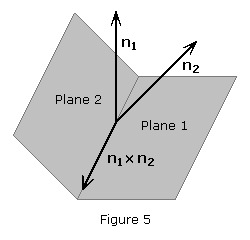
\includegraphics[width=0.6\textwidth]{img/directorrectaimplicitas.jpg}
\caption{Vector director de una recta dada por sus ecuaciones implícitas.}
\label{fig::vectordirectorrectaimplicitas}
\end{figure}

Dada una recta $r$ que pertenece a ambos planos, $\pi_1$ y $\pi_2$, $\vec{v_r}\perp n_{\pi_1} \wedge \vec{v_r}\perp n_{\pi_2}$ (Ver \fref{fig::vectordirectorrectaimplicitas}).
%
Por eso, para buscar un vector perpendiculamr a la vez a 2 vectores dados, el camino más corto es el producto vectorial.

\[\vec{v_r} = n_{\pi_1}\times n_{\pi_2}\]

\begin{problem}

Dada las rectas $r:\left\{\begin{array}{c}2x+y=2\\2y-z=2\end{array}\right.$ y $s:(x,y,z) = (1,1,1) + (-1,2,4)\lambda$.

\solution

Aunque se puede hacer de muchas maneras diferentes, vamos a aplicar el resultado que acabamos de ver.

Los planos que forman la recta $r$ son $\pi_1: 2x+y=2 \text{ con } \vec{n_{\pi_1}} = (2,1,0)$ y $\pi_2: 2y-z=2 \text{ con } \vec{n_{\pi_2}} = (0,2,-1)$ 

Obtenemos $\vec{v_r} = (2,1,0)\times (0,2,-1) = \crossprodandcalc{2}{1}{0}{0}{2}{-1}$

Tenemos $\vec{v_r} \;||\; \vec{v_s}$. Estudiamos $P_s \in r$:

\[
\left\{\begin{array}{c}2·1+1\neq2\\2·1-1\neq2\end{array}\right. \implies P_s\not\in r\implies r\;||\;s \text{ no coincidentes.}
\]
\end{problem}



\obs Fíjate que podríamos haber obtenido $\vec{v_r}$ parametrizando. ¿Cuándo es más corto parametrizar y cuándo utilizar el producto vectorial?

\begin{problem}
Dadas las siguientes rectas, obtén un vector director por el camino más corto

\ppart $r_1:\left\{\begin{array}{c}2x+y=2\\2y-z=2\end{array}\right.$
\ppart $r_2:\left\{\begin{array}{c}2x+5y+z=2\\3x-2y-7z=2\end{array}\right.$
\ppart $r_3:\left\{\begin{array}{c}x+y+z=2\\x-y-z=2\end{array}\right.$

\solution


\end{problem}


\paragraph{Problemas recomendados: T12 - 127,128}

\begin{problem}[Junio 2019]

Dados los puntos $A(1,1,1), B(1,3,-3)$ y $C(-3,-1,1)$, se pide:
\ppart Determinar la ecuación del plano que contiene a los 3 puntos.
\ppart Obtener un punto $D$ (distinto a los anteriores) tal que los vectores $\vec{AB}$, $\vec{AC}$,$\vec{AD}$ sean linealmente dependientes.
\ppart Encontrar un punto $P$ del eje $OX$, de modo que el volumen del tetraedro de vértices $A$,$B$,$C$,$P$ sea igual a 1.

\solution

\spart 

Tomamos $\vec{AB} = (0,2,-4)$, $\vec{AC} = (-4,-2,0)$ como vectores directores del plano y calculamos su ecuación implícita:

\[
\pi: \left|\begin{array}{ccc}
x - 1 & 0 & -4\\
y - 1 & 2 & -2\\
z - 1 & -4& 0
\end{array}\right| = 0 \dimplies 16y-16 + 8z-8-8x+8 = 0\]
\[\dimplies -8x + 16y + 8z -16 = 0 \dimplies -x+2y+z-2=0
\]

\spart Basta con tomar $D\in\pi$. Por ejemplo: $D(0,1,0)\in\pi$.

Comprobamos que $\vec{AB},\vec{AC},\vec{AD}$ son linealmente dependientes calculando el determinante de la matriz que forman.

$\vec{AD} = (1,0,1)$

\[
|\vec{AB}\quad\vec{AC}\quad\vec{AD}| = 
\left|\begin{array}{ccc}
1 & 0 & -4\\
0 & 2 & -2\\
1 & -4& 0
\end{array}\right| = 0
\]

\spart 

(Ojo que aquí no se puede simplificar, aunque antes sí hubiéramos podido)

Buscamos $P(a,0,0)$. El volumen del tetraedro será $\rfrac{1}{6}$ del voluen del paralelepípedo.

\[
\left|\left|\vec{AP}\quad\vec{AB}\quad\vec{AC}\right|\right| = 6 \dimplies
\left|\left|\begin{array}{ccc}
a-1 & 0 & -4\\
-1 & 2 & -2\\
-1 & -4& 0
\end{array}\right|\right| = 2·2·\left|\left|\begin{array}{ccc}
a-1 & 0 & 2\\
-1 & 1 & 1\\
-1 & -2& 0
\end{array}\right|\right| = {6} 
\]
\[
 \left|\left|\begin{array}{ccc}
a-1 & 0 & 2\\
-1 & 1 & 1\\
-1 & -2& 0
\end{array}\right|\right| = \frac{3}{2}  \dimplies |2a+4| = \rfrac{3}{2} \implies\]
\[
\left\{\begin{array}{c}
4+2a_1 = -\rfrac{3}{2} \dimplies a_1 = \frac{-11}{4} \to P_1\left(\rfrac{-11}{4},0,0\right)\\
4+2a_2 = \rfrac{3}{2} \dimplies a_2 = \frac{-5}{4} \to P_2\left(\rfrac{-5}{4},0,0\right)
\end{array}\right.
\]

\end{problem}


\subsection{Proyecciones y simetrías}

\subsubsection{Proyección}

\paragraph{Proyección de punto sobre plano}
\index{Proyección!punto sobre plano}

Para calcular la proyección de un punto $P$ sobre un plano $\pi$ (ver \fref{fig::proy::punto-plano}):
\begin{enumerate}
  \item $r\perp \pi$ con $P\in r$
  \item $P' = r\cap \pi$
\end{enumerate}

\begin{figure}[H]
\centering
\tdplotsetmaincoords{60}{110}

\begin{tikzpicture}[tdplot_main_coords,scale=0.8]
    % draw axes
    \fill[blue!20!white] (-2,-2,0) to (5,-2,0) to (5,5,0) node[anchor=south,color=black]{$\pi$} to (-2,5,0)to cycle;
    \draw[dashed,color=black!45!white] (2,2,-1) -- (2,2,4) node[anchor=west]{$r\perp\pi$};
    \draw[fill] (2,2,3) circle(1pt) node[anchor=west]{$P$};
    \draw[fill,color=red] (2,2,0) circle(1pt) node[anchor=west]{$P'$};
\end{tikzpicture}
\caption{Proyección de punto sobre plano}
\label{fig::proy::punto-plano}
\end{figure}

\paragraph{Proyección de recta sobre plano}
\index{Proyección!recta sobre plano}

Se reduce a proyectar 2 puntos de la recta sobre el plano. Se puede utilizar el punto de intersección de la recta con el plano.

\obs Buenas prácticas: calcular el punto de intersección para saber si la recta pertenece al plano o es paralela. 
\begin{itemize}
  \item Si $r\in\pi$, la proyección de la recta será ella misma.
  \item Si $r\;||\;\pi$, necesitaremos proyectar 2 puntos de la recta.
  \item En los demás casos, se proyecta un punto sobre la recta y la proyección será la que pasa por el punto proyectado y el punto de intersección. Ver \fref{fig::proy::recta-plano}.
\end{itemize}

\begin{figure}[H]
\centering
\tdplotsetmaincoords{60}{110}
\begin{tikzpicture}[tdplot_main_coords,scale=0.8]
    % draw axes
    \fill[blue!20!white] (-2,-2,0) to (6,-2,0) to (6,6,0) node[anchor=south,color=black]{$\pi$} to (-2,6,0)to cycle;
    \draw (0,0,0) -- (2.5,5,5) node[anchor=west]{$r$};
    \draw[dashed] (-1,-2,-2) -- (0,0,0);
    \draw[fill] (0,0,0)circle(2pt) node[anchor=south]{$Q$};
    \draw[fill] (2,4,4)circle(2pt) node[anchor=north west]{$P$};
    \draw[fill] (2,4,0) circle(2pt) node[anchor=north]{$P'$};
    \draw[dashed] (2,4,4) -- (2,4,0);
    \draw[color=red] (-1,-2,0) -- (2.5,5,0) node[anchor=north east]{$r'$};  
\end{tikzpicture}
\caption{Proyección de recta sobre plano}
\label{fig::proy::recta-plano}
\end{figure}


\begin{problem}

Dada la recta $r:\left\{\begin{array}{c}2x+y+z=1\\x+2y+z=2\end{array}\right.$ y el plano $\pi:2x+2y+z=2$, halla la proyección de $r$ sobre $\pi$

\solution

\ul{Cálculo intersección $r\cap\pi$}
\textit{Seguimos el consejo de buenas prácticas.}

\[
\left\{\begin{array}{c}
2x+y+z=1\\
x+2y+z=2\\
2x+2y+z=2
\end{array}\right\} \overset{E_3-E_2}{\dimplies}
\left\{\begin{array}{c}
2x+y+z=1\\
x+2y+z=2\\
x=0
\end{array}\right\} \overset{E_1-E_2}\dimplies 
\left\{\begin{array}{c}
2x+y+z=1\\
x-y=-1\\
x=0
\end{array}\right\}  \dimplies\]\[
\left\{\begin{array}{c}
2x+y+z=1\\
y=1\\
x=0
\end{array}\right\} \to A = \pi\cap r = (0,1,0)\]

Ya tenemos un punto de la recta buscada. Necesitamos hallar la proyección de un $P_r$ sobre el plano.

\ul{Cálculo de proyección de un punto $P_r$}

1) Tomamos $x=1$ y sustituimos en $r$ para hallar $P_r$

\[
\left\{\begin{array}{c}2x+y+z=1\\x+2y+z=2\end{array}\right\}\to
\left\{\begin{array}{c}
y+z=-1\\
2y+z=1
\end{array}\right\}\overset{E_2-E_1}\dimplies
\left\{\begin{array}{c}
y+z=-1\\
y=2
\end{array}\right\}\to (x,y,z) = (1,2,-3)
\]

2) Buscamos $t\perp\pi$ con $P_r\in t$. 

\[
t:\left\{\vec{n_{\pi}},P_r \right\}:\left\{
\begin{array}{c}
x=1+2\lambda
y=2+2\lambda
z=-3+\lambda
\end{array}
\right\}
\]

3) La recta proyección será la formada por $A$ y $B=t\cap\pi$ 

\[
B: 2(1+2\lambda)+2(2+2\lambda)+(-3+\lambda)=2 \dimplies 9\lambda+3=2\dimplies \lambda=\rfrac{-1}{9}
\]

Así, $B\left(1+2\rfrac{-1}{9},2+2\rfrac{-1}{9},-3+\rfrac{-1}{9}\right)$ 

\ul{Conclusión:}
$A (0,1,0)$ y $B\left(\rfrac{7}{9},\rfrac{16}{9},\rfrac{-28}{9}\right)$ forman la recta $r$.


$\vec{AB} = \left(\rfrac{7}{9},\rfrac{7}{9},\rfrac{-28}{9}\right)$. Como $\vec{AB} \;||\; (7,7,-28) \;||\; (1,1,-4)$ tomamos como $\vec{v} = (1,1,-4)$

\[
\text{Solución: }r:\{A,\vec{v}\}:
\left\{\begin{array}{l}
x=\lambda\\
y=1+\lambda\\
z=-4\lambda
\end{array}
\right.
\]
\end{problem}



\paragraph{Proyección de punto sobre recta:}
\index{Proyección!punto sobre recta}

\begin{figure}[H]
\centering
\tdplotsetmaincoords{60}{110}
\begin{tikzpicture}[tdplot_main_coords,scale=0.8]
    % draw axes
    \fill[blue!20!white] (-4,0,-2) to (4,0,-2) to (4,0,4) node[anchor=south,color=black]{$\pi$} to (-4,0,4)to cycle;
    \draw (0,0,0) -- (0,4,0) node[anchor=east]{$r$};
    \draw[dashed] (0,-1.6,0) -- (0,0,0);
    \draw (0,-1.6,0)--(0,-3,0);
    \draw[fill,color=red] (0,0,0)circle(2pt) node[anchor=north]{$P'$};
    \draw[fill] (0,0,3)circle(2pt) node[anchor=west]{$P$};
    \draw[dashed] (0,0,0) -- (0,0,3);
\end{tikzpicture}
\caption{Proyección de punto sobre recta}
\label{fig::proy::punto-recta}
\end{figure}


\begin{problem}
Página 311, ejercicio 11
\solution
\end{problem}

\subsubsection{Simetría de un punto respecto de otro punto}
\index{Simetría!punto respecto de punto}

Todo el cálculo de objetos simétricos respecto de otros se va a basar en este caso, el caso más simple.

\begin{figure}[H]
\centering
\tdplotsetmaincoords{60}{110}
\begin{tikzpicture}[tdplot_main_coords,scale=0.8]
    % draw axes
    %\fill[blue!20!white] (-2,-2,0) to (6,-2,0) to (6,6,0) node[anchor=south,color=black]{$\pi$} to (-2,6,0)to cycle;
    \draw[dashed] (0,3,0) -- (0,0,0);
    \draw[dashed] (0,-3,0) -- (0,3,0);
    \draw[fill,color=red] (0,-3,0)circle(2pt) node[anchor=south]{$P'$};
    \draw[fill] (0,3,0)circle(2pt) node[anchor=south]{$P$};
    \draw[fill] (0,0,0) circle(2pt) node[anchor=south]{$M_{PP'}$};
\end{tikzpicture}
\caption{Simetría de un punto respecto de otro punto}
\label{fig::sim::punto-punto}
\end{figure}


\begin{problem}

Dado el punto $A(2,3,4)$ halla su simétrico respecto de $B(1,1,1)$.

\solution

Buscamos $A'$ que cumpla que $B$ es el punto medio entre $A$ y $A'(x,y,z)$.

Sabemos que el punto medio entre $P$ y $Q$ tiene coordenadas:$M_{PQ}\left(\frac{p_1+q_1}{2},\frac{p_2+q_2}{2},\frac{p_3+q_3}{2}\right)$

Resolvemos:

\[
\left(\frac{2+x}{2},\frac{3+y}{2},\frac{4+z}{2}\right) = (1,1,1) \dimplies ... \dimplies (x,y,z) = (0,-1,-2)
\]

\end{problem}


\subsubsection{Simetría de un punto respecto de una recta}
\index{Simetría!punto respecto de recta}

Plano perpendicular a la recta que contenga al punto, intersección con la recta (ver \fref{fig::sim::punto-recta}).

\begin{figure}[H]
\centering
\tdplotsetmaincoords{60}{110}
\begin{tikzpicture}[tdplot_main_coords,scale=0.8]
    % draw axes
    \fill[blue!20!white] (-4,0,-4) to (4,0,-4) to (4,0,4) node[anchor=south,color=black]{$\pi$} to (-4,0,4)to cycle;
    \draw (0,0,0) -- (0,4,0) node[anchor=east]{$r$};
    \draw[dashed] (0,-1.6,0) -- (0,0,0);
    \draw (0,-1.6,0)--(0,-3,0);
    
    \draw[fill] (0,0,2)circle(2pt) node[anchor=west]{$P$};
    \draw[fill] (0,0,0)circle(2pt) node[anchor=north]{$M_{PP'}$};
    \draw[fill,color=red] (0,0,-2)circle(2pt) node[anchor=west]{$P'$};
    \draw[dashed] (0,0,-2) -- (0,0,2);
\end{tikzpicture}
\caption{Simetría de punto respecto de recta}
\label{fig::sim::punto-recta}
\end{figure}


\subsubsection{Simetría de un punto respecto de un plano}
\index{Simetría!punto respecto de un plano}

Recta perpendicular al plano, que pasa por el punto (ver \fref{fig::sim::punto-plano}).

\begin{figure}[H]
\centering
\tdplotsetmaincoords{60}{110}
\begin{tikzpicture}[tdplot_main_coords,scale=0.8]
    % draw axes
    \fill[blue!20!white] (-2,-2,0) to (5,-2,0) to (5,5,0) node[anchor=south,color=black]{$\pi$} to (-2,5,0)to cycle;
    \draw(2,2,1) -- (2,2,3);
    \draw(2,2,0) -- (2,2,1) node[anchor=west]{$r\perp\pi$};
    \draw[dashed](2,2,-2) -- (2,2,0);
    \draw(2,2,-3) -- (2,2,-2);
    \draw[fill] (2,2,3)circle(1pt) node[anchor=east]{$P$};
    \draw[fill] (2,2,0) circle(1pt) node[anchor=north east]{$M_{PP'}$};
    \draw[fill,color=red] (2,2,-3) circle(1pt) node[anchor=east]{$P'$};
\end{tikzpicture}
\caption{Simétrico de punto respecto de un plano}
\label{fig::sim::punto-plano}
\end{figure}



\subsubsection{Simetría de una recta respecto de un plano}
\index{Simetría!recta respecto de plano}

\begin{figure}[H]
\centering
\tdplotsetmaincoords{60}{110}

\begin{tikzpicture}[tdplot_main_coords,scale=0.8]
    % draw axes
    \fill[blue!20!white] (-2,-2,0) to (6,-2,0) to (6,6,0) node[anchor=south,color=black]{$\pi$} to (-2,6,0)to cycle;
    \draw (0,0,0) -- (2.5,5,5) node[anchor=east]{$r$};
    \draw[dashed] (-1,-2,-2) -- (0,0,0);
    \draw[fill] (0,0,0)circle(2pt) node[anchor=south]{$Q$};
    \draw[fill] (2,4,4)circle(2pt) node[anchor=north west]{$P$};
    \draw[fill] (2,4,0) circle(2pt) node[anchor=north]{$M_{PP'}$};
    \draw[fill] (2,4,-4) circle(2pt) node[anchor=north]{$P'$};
    \draw[dashed] (2,4,4) -- (2,4,-4);
    \draw[color=red] (-1,-2,2) -- (0,0,0);  
    \draw[color=red,dashed] (0,0,0) -- (1.4,2.8,-2.8) node[anchor=north east]{$r'$};  
    \draw[color=red] (1.4,2.8,-2.8) -- (2,4,-4) ;  
\end{tikzpicture}
\caption{Simetría de una recta respecto de un plano}
\label{fig::sim::recta-plano}
\end{figure}


\begin{problem}

Halla la recta simétrica de $r$ respecto del plano $\pi: 2x+2z=0$.

\[r: \begin{cases}x=1+\lambda\\y=1-\lambda\\z=\lambda\end{cases}\]

\solution


\end{problem}


\newpage
\subsection{Ángulos}
\subsubsection{Ángulo formado por dos rectas}
\index{Ángulo!formado por dos rectas}

Llamamos ángulo formado por 2 rectas al menor de los 2 ángulos que forman (en la \fref{fig::ang-recta-recta}, llamaríamos $\widehat{r,s} = \alpha$). Según su posición relativa se distinguen:

\begin{itemize}
  \item \textbf{Secantes:} el ángulo de las rectas será el ángulo de los vectores directores.
  \item \textbf{Paralelas/coincidentes:} ángulo 0.
  \item \textbf{Rectas que se cruzan:} el ángulo que forman es el que forman 2 paralelas a ellas que sean secantes. 
\end{itemize}

Se calcula el ángulo desde la definición de producto escalar.

\[
\cos(\alpha) = \cos(\hat{r,s}) = \left| \cos\left(\hat{\vec{v_r},\vec{v_s}}\right)\right| = \frac{|\vec{v_r}·\vec{v_s}|}{|\vec{v_r}|·|\vec{v_s}|} \implies 0\leq \alpha \leq \rfrac{\pi}{2}
\]


\begin{figure}[H]
\centering
\tdplotsetmaincoords{60}{110}
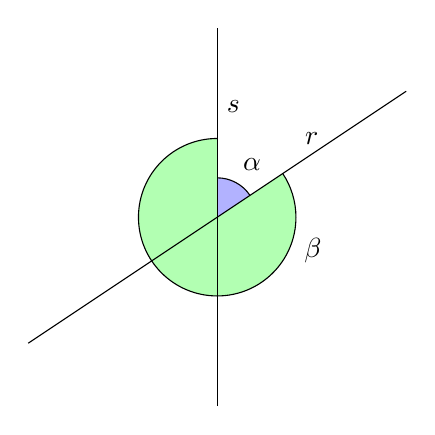
\begin{tikzpicture}[scale=0.8]
    % draw axes
\coordinate (a) at (0,0);
\coordinate (b) at (3,2);
\coordinate (c) at (0,3);

\draw pic[draw,fill=green!30,angle radius=1cm,"$\beta$" shift={(15mm,1mm)}] {angle=c--a--b};
\draw pic[draw,fill=blue!30,angle radius=0.5cm,"$\alpha$" shift={(3mm,4mm)}] {angle=b--a--c};

\draw  (-3,-2) -- (a) -- node[above] {$r$} (b);
\draw  (0,-3) -- (a) -- node[above right] {$s$} (c);
\end{tikzpicture}
\caption{Ángulo formado por 2 rectas}
\label{fig::ang-recta-recta}
\end{figure}


\subsubsection{Ángulo formado por dos planos}
\index{Ángulo!formado por dos planos}

Llamamos ángulo formado por 2 planos al menor de los 2 ángulos diedros que forman 2 planos secantes (ver \fref{fig::ang-plano-plano}).

\obs Si los planos son paralelos, no forman ningún ángulo.

\[
\cos(\alpha) = \cos\left(\widehat{\pi_1,\pi_2}\right) = \left|\cos\left(\widehat{\vec{n_1},\vec{n_2}}\right)\right| = \frac{|\vec{n_1}·\vec{n_2}|}{|\vec{n_1}|·|\vec{n_2}|} \implies 0\leq \alpha \leq \rfrac{\pi}{2}
\]

\begin{figure}[H]
\centering
%\tdplotsetmaincoords{60}{110}
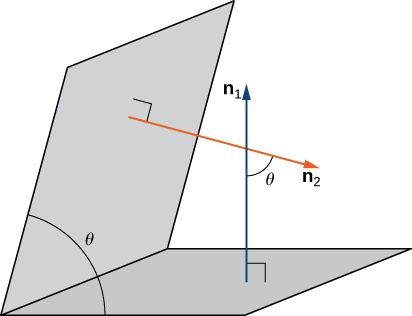
\includegraphics[width=0.6\textwidth]{img/angle-between-planes.jpeg}
%\input{tikz/ang-plano-plano.tex}
\caption{Ángulo formado por 2 planos}
\label{fig::ang-plano-plano}
\end{figure}


\subsubsection{Ángulo formado por recta y plano}
\index{Ángulo!formado por recta y un plano}

\begin{itemize}
  \item Sería posible calcular el ángulo que forma la recta con su proyección. Ver \fref{fig::ang-recta-plano}.
  \item Otra posibilidad, utilizar el vector normal del plano: $\widehat{r,\pi} = 90º-\widehat{r,\vec{n_{\pi}}}$
\end{itemize}


\begin{figure}[H]
\centering
\tdplotsetmaincoords{60}{110}
\begin{tikzpicture}[tdplot_main_coords,scale=0.8]
    % draw axes
    \coordinate (P) at (2,4,4);
    \coordinate (O) at (0,0,0);
    \coordinate (Q) at (2,4,0);

    % draw axes
    \fill[blue!20!white] (-2,-2,0) to (6,-2,0) to (6,6,0) node[anchor=south,color=black]{$\pi$} to (-2,6,0)to cycle;
    \draw (0,0,0) -- (2.5,5,5) node[anchor=east]{$r$};
    \draw[dashed] (-1,-2,-2) -- (0,0,0);
    \draw[fill] (0,0,0)circle(2pt) node[anchor=south]{$Q$};
    \draw[fill] (2,4,4)circle(2pt) node[anchor=north west]{$P$};
    \draw[fill] (2,4,0) circle(2pt) node[anchor=north]{$P_{\pi}$};
    
    \draw[dashed] (2,4,4) -- (2,4,0);


    \draw[color=red,dashed] (-1,-2,0) -- (0,0,0);  
    \draw[color=red,dashed] (0,0,0) -- (1.4,2.8,0) node[anchor=north east]{$r_{\pi}$};  
    \draw[color=red,dashed] (1.4,2.8,0) -- (2.5,5,0); 


    \pic [color=green!30!black,fill=green!30!black,draw, ->, "$\alpha$", angle eccentricity=1.5] {angle = Q--O--P};
    %\fill[color=green!30!black] (0,0,0) -- (-0.5,0,0) -- (-0.635,0.35,0) -- cycle;
\end{tikzpicture}
\caption{Ángulo formado por una recta y un plano}
\label{fig::ang-recta-plano}
\end{figure}

\begin{problem}

Calcula el ángulo formado por la recta $r$ y el plano $\pi$.

\[
r : \begin{cases} 2x-3y+z=0\\x-z=0\end{cases}\;\;\;\pi: x+y-2z=3
\]
\solution

Obtenemos las ecuaciones paramétricas de la recta, calculando las soluciones del sistema compatible indeterminado:

\[
r : \begin{cases} 2x-3y+z=0\\x-z=0\end{cases} \overset{x=\lambda}{\to}
\begin{cases} 2\lambda-3y+\lambda = 0 \to y=\lambda \\x=z=\lambda\end{cases} \dimplies \begin{cases}x=\lambda\\y=\lambda\\z=\lambda\end{cases}
\]

\ul{Método 1: Angulo entre vectores}

\[
\widehat{\pi,\vec{v_r}} = 90 - \widehat{\vec{n_{\pi}},\vec{v_r}}
\]

\[
\cos\left(\widehat{\vec{n_{\pi}},\vec{v_r}}\right) = \frac{|\vec{n_{\pi}}·\vec{v_r}|}{|\vec{n_{\pi}}|·|\vec{v_r}|} = \frac{(1,1,1)·(1,1,-2)}{\sqrt{1^2+1^2+1^2}·\sqrt{1^2+1^2+(-2)^2}} = 0 
\]

\[
\cos\left(\widehat{\vec{n_{\pi}},\vec{v_r}}\right) = 0\implies \widehat{\vec{n_{\pi}},\vec{v_r}} = 90 \implies \widehat{\pi,\vec{v_r}} = 0 \implies \pi\;||\; r
\]


\ul{Método 2: Ángulo con la proyección} (no merece la pena)

Para calcular la proyección de una recta sobre un plano:
\begin{enumerate}
  \item Comprobamos $r\in \pi: \lambda+\lambda-2\lambda = 3 \nexists\lambda\in\real\implies r\;||\;\pi$ con $r\cap\pi=\emptyset$ 
  
  \item Varias opciones:
  \subitem a) Necesitamos proyectar 2 puntos de la recta sobre el plano. Tomamos los puntos $A(0,0,0)\in r$ y $B(1,1,1)\in r$.

  \textbf{$A_{\pi}$:} Calculamos $t\perp\pi (\implies \vec{v_t}\;||\;\vec{n_{\pi}})$ con $A\in t\to t\begin{cases}x=\lambda\\y=\lambda\\z=-2\lambda\end{cases}$

  Calculamos $t\cap\pi: \lambda+\lambda+4\lambda=3\dimplies \lambda=\rfrac{1}{2} \implies t\cap\pi =A_{\pi}=\left(\rfrac{1}{2},\rfrac{1}{2},-1\right)$

  \textbf{$B_{\pi}$:} Calculamos $t'\perp\pi (\implies \vec{v_t'}\;||\;\vec{n_{\pi}})$ con $B\in t'\to t'\begin{cases}x=1+\mu\\y=1+\mu\\z=1-2\mu\end{cases}$

  Calculamos $t'\cap\pi: (1+\mu)+(1+\mu)-2(1-2\mu)=3\dimplies \mu=\rfrac{1}{2} \implies t\cap\pi =B_{\pi}=\left(\rfrac{3}{2},\rfrac{3}{2},0\right)$

  Calculamos $r_{\pi}:\{A,\vec{AB}\} \dimplies r:\begin{cases}x=\rfrac{1}{2}+\lambda\\y=\rfrac{1}{2}+\lambda\\z=\rfrac{1}{2}+\lambda\end{cases}$

\obs ¿Es casualidad que $\vec{v_r} = \vec{v_{r_{\pi}}}$? No, una recta paralela a un plano y su proyección sobre ese plano son rectas paralelas, por lo que tienen vectores directores proporcionales.
\end{enumerate}

\end{problem}



\subsubsection{Perpendicular común}

Ver \fref{fig::Perpendicularcomun}. Buscamos la recta $t$, perpendicular a la vez a $s$ y a $r$, que las corte. 

Para ello:
\begin{itemize}
  \item $\vec{v_t} = \vec{v_r}\times\vec{v_s}$
  \item Dado que encontrar los puntos de intersección es muy complejo, podemos recurrir a construir 2 planos.
  \begin{itemize}
    \item $\pi_1: \{\vec{v_t},\vec{v_r},P_r\}$
    \item $\pi_2: \{\vec{v_t},\vec{v_s},P_s\}$
  \end{itemize}
  Así, $t:\{\pi_1,\pi_2\}$
\end{itemize}

\begin{problem}
Video de unicoos.
\solution

\end{problem}


\begin{figure}[H]
\centering
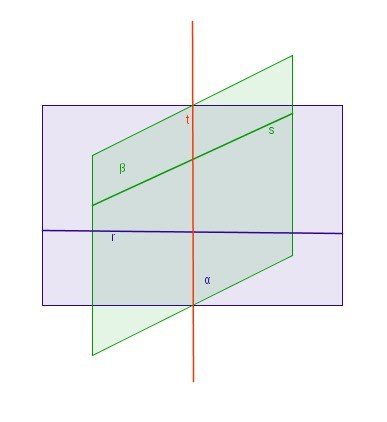
\includegraphics[scale=0.7]{img/PerpendicularComun.jpg}
\caption{Perpendicular común}
\label{fig::Perpendicularcomun}
\end{figure}

\subsubsection{Recta que corta a 2 rectas y pasa por un punto.}

%Vídeo de unicoos para ver en casa (si funciona el anterior).


\subsection{Distancias}
\subsubsection{Entre 2 puntos}
Módulo del vector.

\subsubsection{Entre punto y plano}

La distancia entre el punto y su proyección sobre el plano. Ver \fref{fig::dist-punto-plano}.
\index{Distancia!punto-plano}


\begin{itemize}
  \item $d(P,\pi) = |PP_{\pi}|$, siendo $P_{\pi}$ la proyección del punto sobre el plano.
  \item Se puede utilizar otro camino más corto para calcular esta distancia. Ver \fref{fig::dist-punto-plano}.

  \subitem Consideramos $Q\in\pi$.
  \subitem $|\vec{n_{\pi}}·\vec{QP}| = |\vec{n_{\pi}}|·|\vec{QP}|·\cos(\alpha)$, siendo $\alpha$ el ángulo que forman estos vectores.
  \subitem Aplicando la definición de coseno: $\cos(\alpha) = \rfrac{d(P,\pi)}{|\vec{QP}|}$.
  \subitem Sustituyendo y despejando: $|\vec{n_{\pi}}·\vec{QP}| = |\vec{n_{\pi}}|·d(P,\pi) \to d(P,\pi) = \frac{|\vec{n_{\pi}}·\vec{QP}|}{|\vec{n_{\pi}}|}$
  \subitem $|\vec{n_{\pi}}·\vec{QP}| = |A(p_1-q_1) + B(p_2-q_2) + C(p_3-q_3)| = Ap_1+Bp_2+Cp_3+D$
  \subitem \textbf{Conclusión:}\index{Distancia! punto-plano}

  \[
    d(P,\pi) = \frac{|Aq_1+Bq_2+Cq_3+D|}{|(A,B,C)|}
  \]
\end{itemize}

\begin{figure}[H]
\centering
\tdplotsetmaincoords{60}{110}
\begin{tikzpicture}[tdplot_main_coords,scale=0.8]
    % draw axes
    \fill[blue!20!white] (-2,-2,0) to (6,-2,0) to (6,6,0) node[anchor=south,color=black]{$\pi$} to (-2,6,0)to cycle;
    \draw[->] (0,0,0) -- (2,4,4) node[anchor=south east]{$\overset{\to}{PQ}$};
    \draw[fill] (0,0,0)circle(2pt) node[anchor=south]{$Q$};
    \draw[fill] (2,4,4)circle(2pt) node[anchor=north west]{$P$};
    \draw[fill] (2,4,0) circle(2pt) node[anchor=north]{$P_{\pi}$};
    \draw[->] (0,0,0) -- (2,4,0);
    \draw (1,2,0) node[anchor=north east]{$\overset{\to}{QP_{\pi}}$};
    \draw[dashed] (2,4,4) -- (2,4,0);
    \draw[->,color=red!50!black] (2,4,0) -- (2,4,2) node[anchor=west]{$n_{\pi}$};
\end{tikzpicture}
\caption{Distancia de un punto a un plano}
\label{fig::dist-punto-plano}
\end{figure}


\[d(P,\pi) = \frac{|Ap_1+Bp_2+Cp_3+D|}{|(A,B,C)|}\]

\subsubsection{Entre 2 planos o entre una recta y un plano}
\index{Distancia!plano-plano}
\index{Distancia!recta-plano}

\begin{itemize}
  \item Se comprueba si son paralelos (porque sino, distancia 0).
  \item Si no lo son, calculamos la distancia entre un punto que pertenezca al plano o a la recta y al otro plano.
\end{itemize}


\begin{figure}[H]
\centering
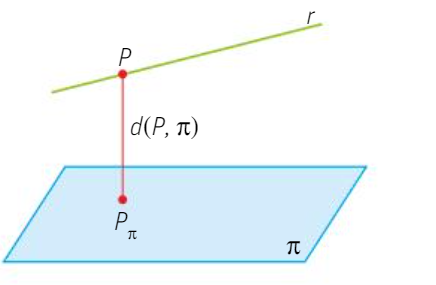
\includegraphics[scale=0.6]{img/dist-recta-plano.png}
\caption{Distancia de una recta a un plano paralelo}
\label{fig::dist-recta-plano}
\end{figure}


\subsubsection{Entre punto y recta}
\index{Distancia!punto-recta}

\begin{itemize}
  \item $d(P,r) = |PP_{r}|$, siendo $P_r$ la proyección de $P$ sobre $r$.
  \item Otra manera de calcular sería considerar un punto $Q\in r$. Ver \fref{fig::dist-punto-recta}.
  \subitem Considerando $\vec{QP}$ y $\vec{v_r}$ (ambos fáciles de calcular), $d(P,r)$ se podría calcular utilizando la definición de seno. Así,
  
  \[\sen\left(\widehat{\vec{v_r},\vec{QP}}\right) = \displaystyle\frac{|d(P,r)|}{|\vec{QP}|}\]

  \subitem Utilizando $|\vec{QP}\times\vec{v_r}| = |\vec{QP}|·|\vec{v_r}|\sen(\alpha)$, despejamos:
  \[
    |\vec{QP}\times\vec{v_r}| = |\vec{QP}|·|\vec{v_r}|·\frac{|d(P,r)|}{|\vec{QP}|} \dimplies d(P,r) = \frac{|\vec{QP}\times\vec{v_r}|}{|\vec{v_r}|}
  \]
\end{itemize}

\begin{figure}[H]
\centering
\tdplotsetmaincoords{60}{110}
\begin{tikzpicture}[scale=1.2]
    % draw axes
    \draw (-3,0) to (3,0) node[anchor=north]{$r$};
    \draw[fill] (-1,0)circle(1pt) node[anchor=south]{$Q$};

    \draw[fill] (1,0)circle(1pt) node[anchor=north west]{$P_{r}$};
    \draw[fill] (1,2)circle(1pt) node[anchor=west]{$P$};
    \draw[->] (-1,0) -- (0,0) node[anchor=north]{$\overset{\to}{v_r}$};
    \draw[->] (1,0) -- (1,2);
    \draw(1,1) node[anchor=west]{$d(P,r)$};
    \draw[->] (-1,0) -- (1,2);
    \draw(0,1.5) node{$\overset{\to}{PQ}$};
\end{tikzpicture}
\caption{Distancia de un punto a una recta}
\label{fig::dist-punto-recta}
\end{figure}



\subsubsection{Entre 2 rectas}
\index{Distancia!recta-recta}
\begin{itemize}
  \item Si $r\cap s \neq \emptyset \implies d(r,s) = 0$
  \item Comprobamos si $r\;||\;s$. 
  \subitem Si $r\;||\;s \implies d(r,s) = d(P_r,s) = d(P_s,r)$
  \subitem Si $r\;\not||\; s \implies d(r,s) = d(r,\pi)$, con $\pi:\{v_r,v_s,P_s\}$
\end{itemize}

\begin{figure}[H]
\centering
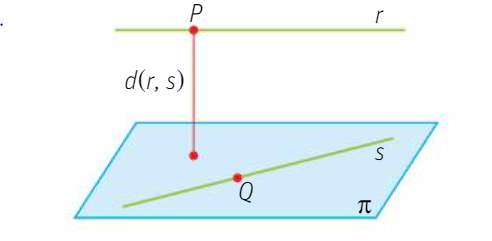
\includegraphics[scale=0.6]{img/dist-recta-recta-cruzan.png}
\caption{Distancia entre 2 rectas que se cruzan}
\label{fig::dist-rectas-cruzan}
\end{figure}


\subsection{Lugares geométricos}


\subsubsection{Plano mediador}

Es el \lgdlp dos puntos $A$ y $B$. Utilizando la definición, consideramos un punto genérico $P(x,y,z)$ al que obligamos a cumplir que 
\[\pi: d(P,A) = d(P,B) \dimplies\]
\[\pi: +\sqrt{(x-a_1)^2+(y-a_2)^2+(z-a_3)^2} = +\sqrt{(x-a_1)^2+(y-a_2)^2+(z-a_3)^2} \dimplies\]
\[\pi: (x-a_1)^2+(y-a_2)^2+(z-a_3)^2 = (x-a_1)^2+(y-a_2)^2+(z-a_3)^2\dimplies ...\]

\paragraph{Otra opción: } Podemos considerar $\pi:\{\vec{AB} = n_{\pi}, M_{AB}\}$ 

\begin{figure}[H]
\centering
\tdplotsetmaincoords{60}{110}
\begin{tikzpicture}[tdplot_main_coords,scale=0.8]
    % draw axes
    \fill[blue!20!white] (-2,-2,0) to (5,-2,0) to (5,5,0) to (-2,5,0) node[anchor=south,color=black]{$\pi_{AB}$} to cycle;
    \draw(2,2,1) -- (2,2,3);
    \draw(2,2,0) -- (2,2,1);
    \draw[dashed](2,2,-2) -- (2,2,0);
    \draw(2,2,-3) -- (2,2,-2);
    \draw[fill] (2,2,3)circle(1pt) node[anchor=east]{$A$};
    \draw[fill] (2,2,0) circle(1pt) node[anchor=north east]{$M_{AB}$};
    \draw[fill] (2,2,-3) circle(1pt) node[anchor=east]{$B$};
    \draw (3,4.5,0) circle(1pt) node[anchor=west]{$P(x,y,z)$};
    \draw[dashed,color=gray] (2,2,3) to (3,4.5,0);
    \draw[dashed,color=gray] (2,2,-3) to (3,4.5,0);
\end{tikzpicture}
\caption{Plano mediador de un segmento.}
\label{fig::plano-mediador}
\end{figure}



\subsubsection{Planos bisectores}

Es el \lgdlp 2 planos $\pi$ y $\tau$. 
%
Utilizando la definición, consideramos un punto genérico $P(x,y,z)$ al que obligamos a cumplir que 

\[d(P,\pi) = d(P,\tau) \dimplies \frac{|A_{\pi}x + B_{\pi}y+C_{\pi}z+D|}{\sqrt{A_{\pi}^2+B_{\pi}^2+C_{\pi}^2}} =  \frac{|A_{\tau}x + B_{\tau}y+C_{\tau}z+D|}{\sqrt{A_{\tau}^2+B_{\tau}^2+C_{\tau}^2}}\]

Dado que $|A| = |B| \dimplies \left\{\begin{array}{c}A=B\\A=-B\end{array}\right\}$, tenemos:

\[
\begin{cases}
\displaystyle\frac{A_{\pi}x + B_{\pi}y+C_{\pi}z+D}{\sqrt{A_{\pi}^2+B_{\pi}^2+C_{\pi}^2}} =  +\frac{A_{\tau}x + B_{\tau}y+C_{\tau}z+D}{\sqrt{A_{\tau}^2+B_{\tau}^2+C_{\tau}^2}}
\\
\displaystyle\frac{A_{\pi}x + B_{\pi}y+C_{\pi}z+D}{\sqrt{A_{\pi}^2+B_{\pi}^2+C_{\pi}^2}} = - \frac{A_{\tau}x + B_{\tau}y+C_{\tau}z+D}{\sqrt{A_{\tau}^2+B_{\tau}^2+C_{\tau}^2}}
\end{cases}
\]

Hay 2 soluciones.

\begin{figure}[H]
\centering
\tdplotsetmaincoords{60}{110}
\begin{tikzpicture}[tdplot_main_coords,scale=0.8]
    % draw axes
    \fill[red!90!white, opacity=0.7] (0,0,0) to (1,0,0) to (1,2,0) to (0,2,0)to cycle;
    \fill[yellow!100!white, opacity=0.9] (1,0,-2) to (1,0,2) to (1,2,2) to (1,2,-2) to cycle;
    \fill[red!90!white, opacity=0.7] (1,0,0) to (2,0,0) to (2,2,0) to (1,2,0)to cycle;
    \draw (1,-0.5,0) to (1,2.5,0) ;
    \draw (1,3,0.5) node{$\to$};
\end{tikzpicture}
\begin{tikzpicture}[tdplot_main_coords,scale=0.8]
    % draw axes
    \fill[blue!20!white, opacity=0.7] (1,0,0) to (0,0,-2) to (0,2,-2) to (1,2,0)to cycle;
    \fill[yellow!100!white, opacity=0.9] (1,0,-2) to (1,0,2) to (1,2,2) to (1,2,-2) to cycle;
    \fill[red!90!white, opacity=0.7] (-0.3,0,0) to (1,0,0) to (1,2,0) to (-0.3,2,0)to cycle;
    %\fill[purple!80!white, opacity=0.7] (1,2,0) to (0,0,1) to (-1,-1,-2) to (1,0,0)to cycle;
    \fill[blue!50!white, opacity=0.7] (1,2,0) to (2,2,-1) to (2,0,-1) to (1,0,0)to cycle;
    \fill[blue!50!white, opacity=0.7] (1,2,0) to (0,2,1) to (0,0,1) to (1,0,0)to cycle;
    \fill[red!90!white, opacity=0.7] (1,0,0) to (2.25,0,0) to (2.25,2,0) to (1,2,0)to cycle;
    \draw (1,-0.5,0) to (1,2.5,0) ;
    \fill[yellow!100!white, opacity=0.9] (1,0,-0) to (1,0,2) to (1,2,2) to (1,2,-0) to cycle;
    \fill[blue!20!white, opacity=0.7] (1,0,0) to (2,0,2) to (2,2,2) to (1,2,0)to cycle;
\end{tikzpicture}
\caption{En azul, olos planos bisectores de un diedro.}
\label{fig::planos-bisectores}
\end{figure}

\begin{problem}
Calcula la ecuación de los planos que dividen a los diedros determinados por los planos $\pi:2x+y-2z=1$ y $\pi': 2x+2y+z=5$ en dos partes iguales.
\solution
Sea $P(x,y,z)$

\[d(P,\pi) = d(P,\pi') \dimplies \frac{|2x+y-2z-1|}{\sqrt{4+1+4}} = \frac{|2x+2y+z-5|}{\sqrt{4+4+1}} \dimplies |2x+y-2z-1| = |2x+2y+z-5|\]

\[
\begin{cases}
2x+y-2z-1 = 2x+2y+z-5\\
2x+y-2z-1 =-\left(2x+2y+z-5\right)
\end{cases}\implies 
\begin{cases}
\tau_1: y+3z-4 = 0\\
\tau_2: 4x+3y-z-6=0
\end{cases}
\]


\obs ¿Qué ángulo forman los 2 planos bisectores? La intuición dice que deberían ser perpendiculares, igual que, en 2 dimensiones, las bisectrices de 2 rectas son perpendiculares. 
%
Vamos a demostrarlo.

\[
\tau_1 \perp\tau_2 \dimplies \vec{n_{\tau_1}} \perp \vec{n_{\tau_2}} \dimplies \vec{n_{\tau_1}}·\vec{n_{\tau_2}} = 0
\]

Comprobamos $\vec{n_{\tau_1}}·\vec{n_{\tau_2}} = (0,1,3)·(4,3,-1) = 3-3=0\implies \tau_1 \perp\tau_2 $

¿Qué ocurre si los planos iniciales, $\pi,\pi'$, son paralelos? En ese caso solo existe un único plano bisector. Vamos a verlo en otro problema diferente.
\end{problem}

\begin{problem}

Determina el lugar geométrico de los puntos del espacio que equidistan de los planos $\pi: x+y+z+4=0$ y $\pi':2x+2x+2z+4=0$.

\solution

Sea $P(x,y,z)$

\[
  d(P,\pi) = d(P,\pi') \dimplies \frac{|x+y+z+4|}{\sqrt{1+1+1}} = \frac{|2x+2y+2z+4|}{\sqrt{4+4+4}} \dimplies 
\]
\[
  \frac{|x+y+z+4|}{\sqrt{3}} = \frac{|2x+2y+2z+4|}{2\sqrt{3}} \dimplies 2·|x+y+z+4| = |2x+2y+2z+4|\dimplies 
\]
\[
\begin{cases}
  2x+2y+2z+8=2x+2y+2z+4 \to \nexists \tau_1\\
  2x+2y+2z+8=-2x-2y-2z-4 \to 4x+4y+4z+12 = 0 \dimplies \tau_2: x+y+z+3=0
\end{cases}
\]

Solo se ha obtenido una solución, debido a que $\pi\;||\;\pi'$.
\end{problem}


\begin{table}[h]
\centering
\begin{tabular}{|c|c|c|}
\hline
\textbf{Definición} & \textbf{Solución} & \textbf{Este curso}\\\hline
2 puntos & Plano mediador & Sí\\\hline
2 plano & Plano bisector & Sí\\\hline
2 rectas paralelas & Plano ¿mediador? & Sí\\\hline
2 rectas que se cruzan & Ver \fref{fig::lgdlp-rectas-cruzan} & No \\\hline
1 puntos & Superficie esférica & Sí, pero no\\\hline
1 recta & Superficie cilíndrica & No\\\hline
1 plano & No tiene solución & \\\hline
\end{tabular}
\caption{\lgdlp...}
\label{tbl::lugaresgeometricos}
\end{table}

\begin{figure}[H]
\centering
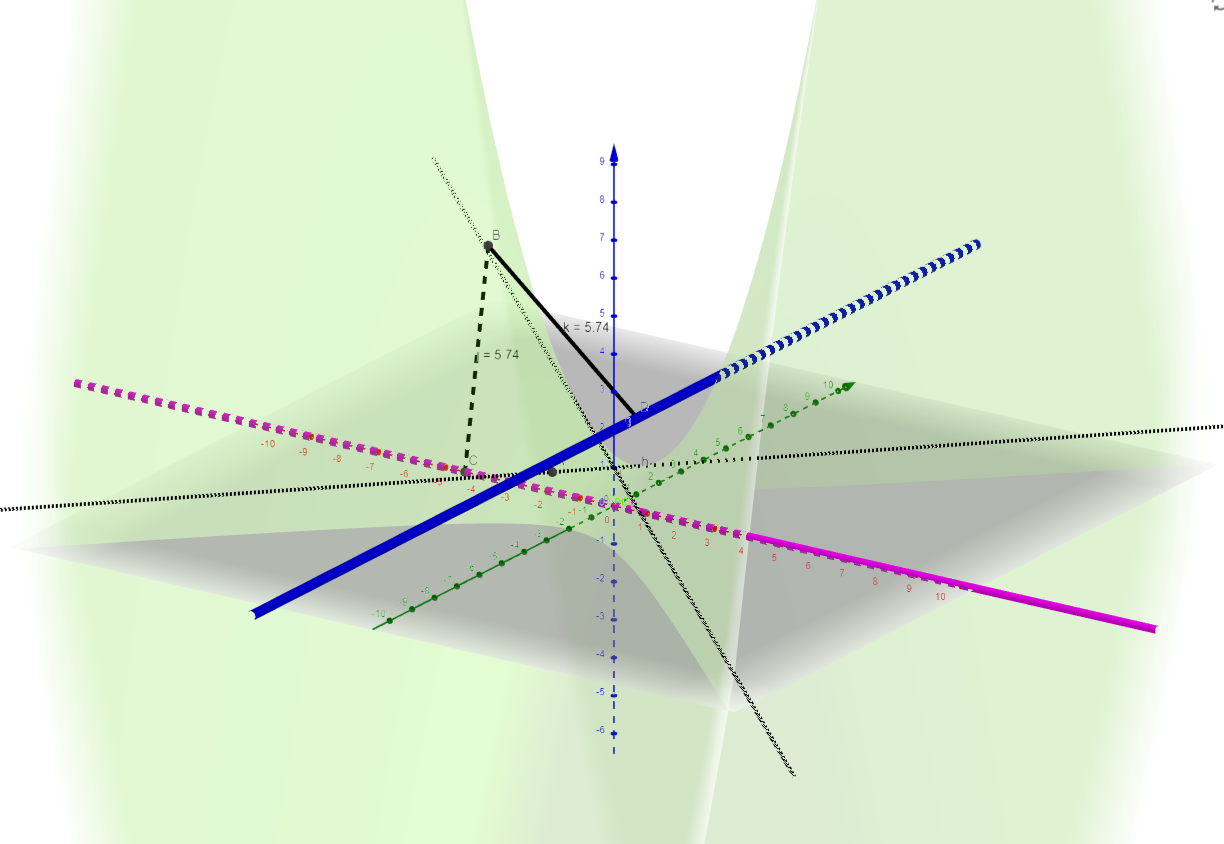
\includegraphics[scale=0.6]{img/lgdlprectascruzan.png}
\caption{Representación geométrica del lugar geométrico de los puntos del epacio que equidistan. Para ver en 3 dimensiones, consultar: https://www.geogebra.org/m/rabpxx8t}
\label{fig::lgdlp-rectas-cruzan}
\end{figure}


\subsection{Áreas y volúmenes}
\begin{itemize}
  \item Área del paralelogramo: $\left|\vec{a}\times\vec{b}\right|$
  \item Área del triángulo: $\rfrac{1}{2}·\left|\vec{a}\times\vec{b}\right|$
  \item Volumen del paralelepípedo: $\left|[\vec{a},\vec{b},\vec{c}]\right|$
  \item Volumen del tetraedro: $\rfrac{1}{6}[\vec{a},\vec{b},\vec{c}]$
\end{itemize}


\begin{problem}
Halla la ecuación de la recta que pasa por el punto $P(2,0,-1)$ y corta a las rectas $r$ y $s$, siendo:

\[r:\frac{x-2}{2} = \frac{y-2}{-1} = \frac{z+1}{1}\]
\[s:\begin{cases}x+y+4=0\\y-3z+3=0\end{cases}\]
\solution
Vídeo de unicoos.

\ul{Plan b:} Método alternativo: mates con Andrés.
\end{problem}


\chapter{Análisis}


\section{Funciones}

El objetivo de esta función es ser capaz de representar gráficas de funciones dada su expresión algebraica. 
%
Para ello vamos a ir desarrollando diferentes herramientas que nos van a resultar tremendamente útiles para este propósito.

\subsection{Concepto}

Lo primero es tener claro qué es una función.

\begin{defn}[Función]
Una función asigna a cada elemento de un conjunto $X$, un único elemento de otro, $Y$. Escribimos $f: X \to Y; x\in X\to f(x)\in Y$
\end{defn}

Ejemplos hablados. Añade 2 de tu propia cosecha.
\begin{itemize}
	\item A cada uno le asigno su edad.
	\item A cada uno su estatura.
	\item A cada uno su brazo.
	\item A un número su doble.
	\item A un número su raíz cuadrada.
\end{itemize}

\begin{itemize}
	\item A un número complejo su conjugado.
	\subitem Sí, pero sólo vamos a hablar de \concept{funciones reales de variable real}. 
\end{itemize}

Escribimos:  $f: D(f)\subset\real \to I\subset\real; x\to f(x)$

\textit{Como curiosidad hay funciones de variable ``funcional'', es decir, que asocia funciones con otras cosas. Este tipo de cosas se estudian en matemáticas.}


\subsubsection{Dominio y recorrido} Condiciones generales de cada función:

$f:\real\to\real\quad\quad D(f) = {x / \exists f(x)}$

Ejemplos:
\begin{itemize}
	\item $f_1(x) = 3x^2+2$
	\item Racionales $f_2(x) = \frac{x+2}{x-1}$
	\item Radicales $f_3(x) = \sqrt{x^2-9}$
	\item Radicales $f_4(x) = \sqrt[3]{x^2-16}$
	\item Exponenciales $f_5(x) = e^x$
	\item Logaritmos $f_6(x) = \log(x+2)$
	\item Trigonométricas $f_7(x) = \cos(x)$
	\item Trigonométricas $f_8(x) = \sin(x)$
	\item Combo: $f_9(x) = \frac{\log(x-5)}{x+7}$
	\item Combo: $f_{10}(x) = \frac{\sqrt{5-x}}{x+7}$
\end{itemize}


\paragraph{Clasificacion de funciones} \textit{Damos la definición formal y la intuitiva.}

\begin{itemize}
	\item Inyectiva: $x\neq y \implies f(x) \neq f(y)  $
	\item Sobreyectiva: $\forall y\in Y \exists x\in X / f(x) = y$
	\item Biyectiva: sobreyectiva e inyectiva a la vez.
\end{itemize}

\concept{Gráfica de una función:} $G(f) = {\left(a,f(a)\right)}$

\subsection{Operaciones con funciones}
\begin{itemize}
	\item Suma, resta $(f\pm g)(x) = f(x) \pm g(x)$
	\subitem $D(f\pm g) = D(f)\cap D(g)$.
	\item Producto
	\subitem $D(f·g) = D(f)\cap D(g)$.
	\item Cociente 
	\subitem $D\left(\rfrac{f(x)}{g(x)}\right) = D(f)\cap D(g) \setminus \{x/g(x) = 0\}$
	\item Composición $(g\circ f)(x) = g\left(f(x)\right)$ y se lee ``f compuesta con g''.
	\subitem El dominio se recalcula.
\end{itemize}

\concept{Función inversa} $f^{-1}(x):Y\to X$ y cumple $(f\circ f^{-1})(x) = x$

\paragraph{Ejemplo:} Comprueba si son inversas
\begin{itemize}
	\item $f(x) = x^3-1$; $f^{-1}(x) = \sqrt[3]{x+1}$ (sí)
	\item $f(x) = x^2+1$; $f^{-1}(x) = \sqrt{x}$ (no)
\end{itemize}

\paragraph{Ejemplo:} Calcula la función inversa de $f(x) = \frac{2x+1}{3}$ y de $g(x) = \frac{-1}{3x}$ 

\hl{13/03} Corregir pregunta: ¿son funciones inversas?

Construir funciones inversas.

\subsubsection{Clasificacion de funciones}

\begin{defn}[Inyectividad]
$f(x) : D(f) \to \real$ inyectiva $\dimplies\forall a,b\in D(f) a\neq b \implies f(a) \neq f(b)$
\end{defn} 

\begin{defn}[Sobreyectividad]
	$f(x) : D(f) \to \real$ sobreyectiva $\dimplies \forall b\in\real \exists a\in D(f) \tlq f(a) = b$

	Es decir, una función es sobreyectiva si su imagen son todos los números reales.
\end{defn}


\begin{defn}[Biyectividad] 
	Inyectividad y sobreyectividad
\end{defn}

\paragraph{Ejemplos:} Razonando gráficamente.

\begin{itemize}
	\item $f(x) = x^3$ (biyectiva)
	\item $f(x) = x^2$ (nada)
	\item Dibujo función cúbica sí sobreyectica, no inyectiva.
	\item $f(x) = e^x$ (inyectiva)
	\item $f(x) = \log(x)$ (inyectiva)
\end{itemize}

\obs Una función no inyectiva no puede tener inversa.

\section{Continuidad}
\subsection{Límites}

\subsubsection{Repaso de límites de 4º}

\paragraph{Introducción}

Con el excel y geogebra. Definición intuitiva de límite. \textit{Reto: escribe tu propia definición de límite y vete hablándola conmigo.}

\begin{itemize}
	\item Excel: valor del límite: me voy acercando sin llegar a tocar.
	\item Geogebra: mismo gráficamente. Hacer zoom hasta la saciedad.
\end{itemize}

\begin{defn}[Límite en un punto finito]
Sea $f(x):\real\to\real$.

\[\lim_{x\to a} f(x) = b\]

El límite de la función $f(x)$ en un punto $x=a$ es el valor $b$ al que se aproxima la función cuando la variable se aproxima al punto, sin \hl{nunca} alcanzarlo.
\end{defn}

Ejemplos:
\begin{itemize}
	\item $\lim_{x\to 3} x^2 + 1 = 10$
	\item $\lim_{x\to 0} \frac{\sin x}{x} = 1$ (cálculo con calculadora) ¿Existe la función en el punto? Nooooo ¿Existe el límite? Siiiii.
	\item $\lim_{x\to 0} \frac{1}{x^2}$ (cálculo con calculadora). ¿Existe la función en el punto? Nooooo ¿Existe el límite? Puede existir. Decimos que es $\pm\infty$.

\obs Puede ser que la función no se acerque a ningún valor, sino que cada vez se haga más grande. En ese caso el resultado del límite será $+\infty$.

\obs Puede ser que la función no se acerque a ningún valor, sino que cada vez se haga más pequeño. En ese caso el resultado del límite será $-\infty$.
\end{itemize}


\paragraph{Infinito, ¿concepto o valor?}
\subparagraph{Aritmética del infinito}

\hl{Empezar aquí}

\begin{defn}[Límite en el infinito]
Sea $f(x):\real\to\real$.

\[\lim_{x\to \pm\infty} f(x) = b\]

El límite de una función $f(x):\real\to\real$ en el infinito ($\pm\infty$) es el valor $b$ al que se aproxima la función cuando la variable toma valores \hl{arbitrariamente} grandes (o pequeños).
\end{defn}

\obs Se cumplen las mismas observaciones de antes.

\begin{example}
	\[\lim_{x\to\infty}x=\infty\]
	\[\lim_{x\to\infty}\frac{1}{x}=0\]
\end{example}

\begin{defn}[Exsitencia del límite en un punto finito] 
	El límite existe si existen y son iguales los límites laterales. 
\end{defn}


\paragraph{Propiedades de los límites} (me lo he saltado).

Sea $a\in\real\cup\{\infty,-\infty\}$, $f,g:\real\to\real$ y que dado $a$, $\exists\lim_{x\to a}f(x) \;;\; \exists\lim_{x\to a}g(x)$
\begin{itemize}
	\item $\lim_{x\to a} \left(f(x) \pm g(x)\right) = \lim_{x\to a} f(x) \pm \lim_{x\to a} g(x)$
	\item $\lim_{x\to a} \left(f(x) · g(x)\right) = \lim_{x\to a} f(x) · \lim_{x\to a} g(x)$
	\item $\lim_{x\to a} \left(f(x) \pm g(x)\right) = \lim_{x\to a} f(x) \pm g(x)$
	\item $\lim_{x\to a} \left(\frac{f(x)}{g(x)}\right) = \lim_{x\to a} f(x) \pm g(x)$
	\item $\lim_{x\to a} \left(f(x)\right)^{g(x)} = \left(\lim_{x\to a} f(x)\right)^{\lim_{x\to a} g(x)}$	
	\item $\lim_{x\to a} (f\circ g)(x) = ?$	
\end{itemize}

\begin{example}
\[\lim_{x\to 0}\frac{1}{x}\]
 \[\lim_{x\to 4}\left(\frac{x+1}{x}\right)^{\frac{1}{x-4}}\]
\end{example}

\paragraph{Indeterminaciones}

\begin{itemize}
	\item $k/0$
	\subitem Vistas (la $h$). Son indeterminaciones a medias, ya que sólo tienen 2 posibilidades: $\pm∞$
	\item $\infty/\infty$ (potencia más alta del denominador)
	\subitem $\displaystyle\lim_{x\to∞}\frac{x^2+5x+6}{x+\sqrt{x}} = \lim_{x\to∞}\frac{\frac{x^2}{x}+5\frac{x}{x}+\frac{6}{x}}{\frac{x}{x}+\sqrt{\frac{x}{x^2}}} = \lim_{x\to∞}\frac{x+5+\rfrac{6}{x}}{1+\frac{1}{\sqrt{x}}} = ∞$
	\item $0/0$ (simplificar)
	\subitem $\displaystyle\lim_{x\to1}\frac{x^2-5x+4}{x-1}$
	\subitem $\displaystyle\lim_{x\to1}\frac{x-1}{\sqrt{x-1}}$
	\item $\infty-\infty$
	\subitem $\displaystyle\lim_{x\to-∞}x^2+x = \lim_{x\to-∞} x(x+1) = (-∞)·(-∞) = ∞$
	\subitem El problema viene con 

	$\displaystyle\lim_{x\to∞}\sqrt{x^2+1}-x = \lim_{x\to∞}\frac{(\sqrt{x^2+1}-x)(\sqrt{x^2+1}+x)}{\sqrt{x^2+1}+x} = \lim_{x\to∞} \frac{x^2+1-x^2}{\sqrt{x^2+1}+x} = 0$
	\item $1^{+\infty}$
		\subitem Estas indeterminaciones aparecen cuando $\displaystyle\lim_{x\to a}f(x)^{g(x)}\;\lim_{x\to a}f(x) = 1\;\lim_{x\to a}g(x) = ∞$ y se resuelven utilizando:
		\[
			\displaystyle\lim_{x\to a}f(x)^{g(x)} = e^λ, \text{ donde } λ = \lim_{x\to a} (f(x)-1)g(x)
		\]
		\subitem $\displaystyle\lim_{x\to \infty}\left(\frac{x-1}{x}\right)^x = e^λ$ donde $λ=\displaystyle\lim_{x\to∞}\left(\frac{x-1}{x}-1\right)·x = -1$
\end{itemize}

\subsection{Continuidad}

\begin{defn}[Continuidad\IS en un punto]

Una función $f(x):ℝ\toℝ$ es continua en un punto $a$ si y sólo si se cumplen:
\begin{itemize}
	\item $\displaystyle∃\lim_{x\to a}f(x)$
	\item $\displaystyle∃f(a)$
	\item $\displaystyle\lim_{x\to a}f(x) = f(a)$
\end{itemize}

\obs Normalmente diremos: si existen y son iguales el límite y el valor en el punto.
\end{defn}

\paragraph{Tipos de discontinuidades}

Explicar gráficamente los casos.s

\begin{example}
\begin{itemize}
	\item ¿Es continua la función $f(x)= \frac{x^2-1}{x-1}$ en $x=2$?
	\item ¿Es continua la función $f(x)$ en $x=1$? 
	\item ¿Es continua la función $f(x) = \sqrt{x}$ en $x=0$?
	\item Funciones definidas a trozos (hasta aquí).
\end{itemize}
\end{example}

\begin{defn}[Continuidad\IS en un intervalo abierto]
Una función $f(x):ℝ\toℝ$ es continua en $(a,b)\inℝ$ si es continua $∀c\in(a,b)$.
\end{defn}

\begin{itemize}
	\item ¿Es continua la función $f(x) = \frac{x^2-1}{x-1}$ en $(2,∞)$?
	\item ¿Es continua la función $f(x) = \sqrt{x}$ en $(0,∞)$?
\end{itemize}



\begin{example}
Estudia la continuidad de la función $f(x) = \frac{\sqrt{x}}{x-4}$

\obs Una función sólo puede ser continua en su dominio. En este caso: $D(f) = \{x\inℝ\tq x≥0\}-\{x\in\real\tq x-4=0\} = [0,∞)-\{4\}$

La función es continua en $(0,4) ∪ (4,∞)$

\end{example}

\section{Derivabilidad}

\begin{defn}[Derivada\IS en un punto]
Sea $\appl{f}{ℝ}{ℝ}$ una función continua. Se define la derivada de $f$ en el punto $a$ como:

\[
	f'(a) = \lim_{x\to a}\frac{f(x)-f(a)}{x-a}
\]
\end{defn}

\obs $f$ \concept[Función\IS derivable]{derivable} en $x=a \dimplies \exists f'(a)$
\obs A la función inicial la llamaremos primitiva.

\begin{example}
Cálculo de la derivada de $f(x) = x^2+2x-1$ en $x=3$.

\[
	f'(3) = \lim_{\x\to3}\frac{x^2+2x-1 - (3^2+2·3-1)}{x-3} = \lim_{\x\to3}\frac{x^2+2x-15}{x-3} = \lim_{\x\to3}\frac{(x-3)(x+5)}{x-3} = \lim_{\x\to3}(x+5) = 8
\]

\end{example}

\begin{example}
Cálculo de la derivada de $f(x) = |x|$ en $x=0$.

\[
	f'(0) = \lim_{x\to0}\frac{|x| - |0|}{x-0} = \lim_{x\to0}\frac{|x|}{x} = \left\{\begin{array}{l}\displaystyle\lim_{x\to0^+}\frac{x}{x} = 1 \\ \displaystyle\lim_{x\to0^-}\frac{-x}{x}=-1\end{array}\right\}\implies \nexists\lim_{x\to0}f(x)
\]

Conclusión: La función $f(x)$ no es derivable en $x=0$. ¿Es continua? Sí.
\end{example}

\begin{example}
Cálculo de la derivada de $f(x) = \frac{1}{x}$ en $x=0$.

\[
	f'(0) = \nexists\lim_{x\to0}\frac{\rfrac{1}{x}-\rfrac{1}{0}}{x-0}
\]

No es derivable. ¿Es continua? No.
\end{example}

\obs \textbf{Derivable} $\implies$ \textbf{Continua}. \textit{Para que una función sea derivable en un punto es necesario que sea continua en ese punto}\footnote{Está en su tabla de derivadas}.

¿En física habéis derivado polinomios? ¿Cuál sería la "derivada" del polinomio? $f'(x) = 2x+2$. ¿Cuánto vale $f'(3)$? $f'(3) = 2·3+2=8$. ¿Casualidad?

Pero... ¿porqué esto es cierto? ¿De dónde sale ese $3x^2+2$? Esto es a lo que llamamos la función derivada:

\begin{defn}[Función\IS derivada]
Sea $\appl{f}{ℝ}{ℝ}$ una función continua. Se define la función derivada de $f$ como la función que a cada punto le asigna el valor de su derivada.

\[
	f'(x) = \lim_{h\to 0}\frac{f(x+h)-f(x)}{h}
\]
\end{defn}

\begin{example}
Cálculo de la función derivada $f'(x)$ de un polinomio, por ejemplo $f(x)=x^2+2x-1$

\[
	f'(x) = \lim_{h\to0}\frac{f(x+h)-f(x)}{h} = \lim_{h\to0}\frac{(x+h)^2+2(x+h)-1 - x^2+2x-1}{h} =
\]
\[
	\lim_{h\to0}\frac{(x^2+2xh+h^2+2x+2h-1 - x^2-2x+1}{h} = \lim_{h\to0}\frac{2xh+h^2+2h}{h} =
\]
\[
	\lim_{h\to0}\frac{h(2x+h+2)}{h} = \lim_{h\to0} 2x+h+2) = 2x+2
\]

Conclusión: la función derivada de $f(x) = x^2+2x-1$ es $f'(x) = 2x+2$.
\end{example}

\paragraph{Propiedades de la derivada:}
\begin{prop}[Cálculo operativo]
	Sean $f, g$ derivables en $a$. Entonces
	\begin{itemize}
		\item $(k·f(x))' = k·f'(x) ∀k\in\real$
		\item $(f\pm g)'(a)=f'(a)\pm g'(a)$
		\item $(fg)'(a)=f'(a)g(a)+f(a)g'(a)$
		\item Si $g(a)\neq 0 $, $\left(\frac{1}{g}\right)'(a)=\frac{-g'(a)}{(g(a))^2}$
		\item Si $g(a)\neq 0$, $\left(\frac{f}{g}\right)'(a)=\frac{f'(a)g(a)-f(a)g'(a)}{(g(a))^2}$
		\item $(g\circ f)'(a)= g'(f(a))f'(a)$
	\end{itemize}
\end{prop}

\hl{Explicación de la tabla de derivadas}

\paragraph{Regla de la cadena}

\paragraph*{A practicar:}
\begin{itemize}
	\item $\displaystyle f(x) = x\sqrt[3]{x^2}$
	\item $\displaystyle f(x) = x·e^x$
	\item $\displaystyle f(x) = x·\sen(x)$
	\item $\displaystyle f(x) = x·\ln(x)$
	\item $\displaystyle f(x) = \sen(x)·\cos(x)$
	\item $\displaystyle f(x) = \frac{x^2+1}{x}$
	\item $\displaystyle f(x) = (x^2+2x)·\sen(x)$
	\item $\displaystyle f(x) = (e^x - x)·\ln{x}$
	\item $\displaystyle f(x) = \sqrt{x^2+x}$
	\item $\displaystyle f(x) = (\arcsen{x})^3$
	\item $\displaystyle f(x) = \ln(4x)$
	\item $\displaystyle f(x) = (\cos{x})^2 = \cos^2{x}$
	\item $\displaystyle f(x) = \sen{(3x^2)}$
	\item $\displaystyle f(x) = \cos{(x^2+1)} $
	\item $\displaystyle f(x) = \tg{(x^2-3x)}$
	\item $\displaystyle f(x) = \sen{\sqrt{x^2+3x}} $
	\item $\displaystyle f(x) =  \cos{\frac{x-1}{x}}$
	\item $\displaystyle f(x) = \tg{\sqrt{x-1}} $
	\item $\displaystyle f(x) = -\sen{\frac{x}{-x^4+x-1}} $
	\item $\displaystyle f(x) = \tg{\frac{2}{\sqrt{1-x}}} $
\end{itemize}

\subsection{Interpretación geométrica de la derivada}



\section{Integrales inmediatas}



\section{Estudio sistemático de una función}

\begin{itemize}
	\item Dominio, siempre.
	\item Puntos de corte con los ejes.
	\item Simetría.
	\item Asíntotas, repaso de 4º.
	\item Monotonía.
	\item Curvatura.
\end{itemize}

\subsection{Monotonía}

Diferenciar los intervalos en los que la función crece de aquellos en los que la función decrece. También, ¿dónde están los máximos y los mínimos?

\begin{itemize}
	\item Ejemplo: dada la función $f(x) = 3x^2+2x+5$, encuentra sus extremos relativos.
	\item Los extremos relativos se encuentran en los puntos donde la derivada se hace 0. ¿Por qué? Interpretación gráfica.
	\item ¿Cómo distinguir máximo de mínimo? En este caso, la parábola va hacia arriba, por lo que debe ser mínimo. 
	\subitem Por un lado negativa (función decrece), por otro positiva (función creciente).
	\subitem Segunda derivada positiva, lo que marca que es un mínimo.
	\item Concavidad: segunda derivada positiva -> mínimo, convexa.
\end{itemize}

\begin{itemize}
	\item $f'(x) > 0 \implies f(x)$ crece. 
	\item $f'(x) < 0 \implies f(x)$ decrece. 
	\item $f'(x) = 0 \implies $ extremo relativo. ¿Máximo, mínimo?
	\item $f''(x) > 0 \implies $ mínimo y convexa-contenta (desde el semieje negativo de $y$).
	\item $f''(x) < 0 \implies $ máximo y cóncava desde el semieje negativo de $y$.
	\item 
\end{itemize}

Clase del jueves:

\begin{itemize}
	\item Corregir: demuestra que el vértice de la parábola es $\rfrac{-b}{2a}$
	\item Halla las rectas tangentes a la función $f(x)$ en los máximos (no es necesario intervalos de crecimiento y decrecimiento).
	\[
		f(x) = 3x^4-4x^3-36x^2
	\]
	\item Estudia la monotonía (intervalos de crecimiento, decrecimiento y extremos relativos y absolutos) de $f(x) = x^4-2x^2$
	
	\item Estudia sistemáticamente la función: $f(x) = \frac{2(x-2)+1}{(x-2)^2} = \frac{2x-1}{x^2-4x+4}$
	\subitem Punto de corte eje x: $(1.5,0)$, eje y: $(0,-0.75)$, mínimo absoluto: $(1,-1)$
	
	\item Estudia las asíntotas de $f(x) =\frac{x^3-4x^2+x+6}{2x^3-14x^2+32x-24}$
	
	\item Deriva $f(x) = \tan(x^2-3x)$
\end{itemize}

\newpage
\printindex
\listoffigures
\listoftables

\end{document}
